\documentclass[conference]{IEEEtran}
\IEEEoverridecommandlockouts
% The preceding line is only needed to identify funding in the first footnote. If that is unneeded, please comment it out.
\usepackage{cite}
\usepackage{amsmath,amssymb,amsfonts}
\usepackage{algorithmic}
\usepackage{graphicx}
\usepackage{textcomp}
\usepackage{xcolor}
\def\BibTeX{{\rm B\kern-.05em{\sc i\kern-.025em b}\kern-.08em
    T\kern-.1667em\lower.7ex\hbox{E}\kern-.125emX}}
\begin{document}

\title{Private Protection in Generative Models\\
\thanks{University of Science and Technology of China}
}

\author{\IEEEauthorblockN{Haihan Gao}
\IEEEauthorblockA{\textit{SA22011017} \\}
\and
\IEEEauthorblockN{Xiaolu Chen}
\IEEEauthorblockA{\textit{SA22221005} \\}
\and
\IEEEauthorblockN{Li Zhang}
\IEEEauthorblockA{\textit{SA22221064} \\}
}

\maketitle

\begin{abstract}
With the arrival of Big Data Age, machine learning is becoming a hit and at the same time multiple type of information is used for intelligent service. However, some sensitive data is exposed to public without any protection which brings troubles even security risks to data owners. To solve the problem, generative models are used in privacy protection with generating fake data from the distribution of real data so that it can replaced the real privacy data in practice. Although they have been widely used, they still result in inevitable privacy leakage due to their structure characteristics. Some impressive works combining the differential privacy mechanism have been done to provide more data privacy security. The differential privacy is one of the most popular techeniques for privacy protection, Despite of the exploration in the field of privacy preserving, generative models are still faced with several open challenges waiting for solution. It is clear that generative models are good tools to contribute a solution for privacy preserving, but there is still a long way to go.
\end{abstract}

\begin{IEEEkeywords}
privacy protection, privacy preserving, generative model, differential privacy
\end{IEEEkeywords}

\section{Introduction}
In the era of information, data means everything. The promotion of network equipment and applications produces tremendous data which may reveal the latent relationship between things, and because of this data is called another form of wealth. Machine learning is one of the technology based on big data whose boosting development in  greatly brings artificial intelligence more application in practice in many areas such as finance, medical, security and so on. As well as the progress in computing ability and algorithm, data of large amount is also the significant affection contributing to machine learning.

However, some of the collected data for machine learning is sensitive and individual that may cause serious problems not only for data owners but also the public if used maliciously. As a result, researches are attracting public attention which is about how to find a solution to balance data privacy and utility. Some turn to generative models and several outstanding works have been proposed with excellent performance.

\subsection{Importance of Privacy}
It is a pity that there is still no exact definition for privacy data and that increases the difficulty for promoting privacy preserving. For convenience of following statement, we make use of widely accepted concept of privacy that privacy data denotes the sensitive information which its owner is reluctant to offer to public for it is highly closely related to one's identity and interest.

The leakage of privacy not only damages the interests of individuals, but also endangers national security and social stability. Privacy usually plays a role of identity characteristic and it means its closure not only interferes with the normal daily life of public individuals, but also increases the risk of information being misused in illegal ways and infringes the interests of information owners. Besides, Privacy leakage as well harms national security. It is not difficult to realize that malicious groups can collect privacy data for analysis so as to obtain state confidential information, which is taken advantage of to undermine public order and combat government prestige causing threat to the stability of its rule.

It is precisely because of the seriousness of the harm of privacy leakage that individuals and groups are paying more attention to privacy security. The US, the EU, China and other countries are constantly improving data security and privacy protection laws and regulations to regulate enterprises and individuals, such as Privacy Act of US, GDPR of EU and Personal Information Protection Law of China.

\subsection{Techniques for Privacy Preserving}
Despite of the strength of law, users are worried about their information security yet, so they may hesitate when asked to provide their data for formal use like enhancing the function of network service. It may lead to another extreme that data for developing machine learning are becoming less and less. In order to balance the utility and privacy of data, a great number of works have been done.\cite{b1}

\subsubsection{Data Generalization}
By replacing the original data with more general symbol, the sensitive of real data might be weakened, resulting that the statistical characteristics of the sample population will not be changed, as well the sample individuals will not be exposed. K-Anonymity, L-diversity together with their variants can be regarded as the typical works.

\subsubsection{Noise Disturbance}
Adding noise to data is another useful way to hide privacy information when queries come. After adding little noise into the dataset, all privacy data is covered so in the respose to queries the chance of leakage information is quite low. Differential privacy is the representative work which is even the most popular privacy preserving method.

\subsubsection{Data Encryption}
Encryption is a kind of traditional methods to keep the confidentiality of data, also can be used in privacy protection. With the development of cryptography and technology, it has more applications in reality practice such as homomorphic encryption and secure multiparty computation. It is usually used in the scenarios of data exchange or of data separative distribution.

\subsubsection{Generative Fake Data}
Generative models in machine learning provide another way to protect privacy. A generative model can produce new data which is highly similar to the real one without exposing the real original figure to data collectors. Given the generated fake data, there is no need to use real privacy data for it can be replaced. Nowadays, more and more work of this part is emerging.

Under the rapid advancement of machine learning, generative models might be one of the most promising technology for privacy preserving. However, due to their training principle, generative models are limited in maintaining some same features with original data when producing the new, which may cause a great possibility of divulging private information when faced with attack realized in a machine learning way. To enhance the ability of generative models, researchers turn to differential privacy for improvement in efficient guarantee.

\section{Principle of Differential Privacy}
Before the introduction of generative models based on differential privacy mechanism, it is necessary to have acquaintance of differential privacy. The principle of the mechanism is quite simple that when a query is coming, a random noise is added to the dataset which might change the real distribution but keep the whole statistic response to query the same as before, so the it is hardly to tell if the target privacy data is in the dataset. Details about this important privacy preserving technique are presented in following parts.

\subsection{Definition of Differential Privacy}
It is noted that randomization is essential in differential privacy, so several definitions about randomized algorithms ought to be given before a better description of differential privacy.\cite{b2}

In general, a randomized algorithm is able to map a domain to a discrete probability simplex which represents the probability distribution of a range. It is defined as:
\begin{equation}
    M: A \longrightarrow \Delta(B).
\end{equation}
For a randomized algorithm $M$, on input $a \in A$ it outputs $M(a) = b \in B$ with a probability of $(M(a))_b$ for each $b \in B$. Outputs for all inputs are combined as $\Delta(B)$, a probability distribution set denoted:
\begin{equation}
    \Delta(B) = \{x \in R^{|B|}: x_i \geq 0, \sum_{i=1}^{|B|} = 1 \}.
\end{equation}
The difference between datasets is also need defined in differential privacy, so $l_1$ norm is introduced:$||D - D'||_1$ is used to describe how many pieces of data differ in dataset $D$ and $D'$. It is noted that if there is only one piece of data different, $D$ and $D'$ are neighbouring dataset.

Differential privacy can be presented that a randomized algorithm performs similarly on two similar datasets. A randomized algorithm $M$ is $(\sigma,\delta)-differential \quad privacy$, if it follows the given formal definition:
\begin{equation}
    Pr[M(D) \in S] \leq exp(\epsilon) Pr[M(D) \in S] + \delta,
\end{equation}
where $S \subseteq range(M)$. Here $\epsilon$ is called privacy budget which is consumed when dealing with queries. Smaller $\epsilon$ means better privacy protection, but noise added to data is bigger which may lead to the reduction of the data usability. $\delta$ is a relaxation term which is usually smaller than $1/|D|$ allowing little difference between the outputs of the algorithm works on two dataset, and when $\delta = 0$, it is said that $M$ is $\epsilon-differential \quad privacy$.

Differential privacy has three key properties: privacy post-processing, composability of privacy and group privacy.[3] Privacy post-processing means that an algorithm following $(\epsilon,\delta)-differential \quad privacy$ will not be affected by whatever post process applied on the result it computes, so it can be used as a part in any other algorithm. Composability of privacy provides a chance for modular design of mechanisms: if all the components of a mechanism are following differential private, then so is their composition.Take an example, $M_1$ is $\epsilon_1-differential \quad privacy$ and $M_2$ is $\epsilon_2-differential \quad privacy$, while as their composition, $M_12$ is $(\epsilon_1 +\epsilon_2)-differential \quad privacy$,and this also shows privacy preserving reduction. On the other hand, group privacy also causes the strength of the privacy guarantee drops linearly with the size of the group, as the fact that any $(\epsilon,0)-differential \quad privacy$ mechanism is $(k\epsilon,0)-differential \quad privacy$ for group whose size is $k$. Because of these quantities, the composition of differential privacy mechanisms should be designed carefully to achieve higher privacy protection in different circumstances.

\subsection{Differential Privacy Mechanism}
With the exploration going deep into the field of differential privacy, some basic techniques are summarized by researchers, which are regarded as the basic building blocks for developing all other algorithms.

\subsubsection{Randomized Response}
Randomized response mechanism is applied on the non-numerical data. When faced with a yes-or-no query, the response is asked to answer honestly at a probability of $p$, or answer "yes" or "no" randomly at a probability of $1-p$, and "yes" appears at a probability of $q$. The intuition behind randomized response is that it provides "plausible deniability", and in other words, privacy is obtained by process the response of a great group not the exact answer of a person. When $p$ and $q$ depand on coin flipping, this mechanism follows $(ln3,0)-differential \quad privacy$ which is described as:
\begin{equation}
    \begin{split}
        \frac{Pr[response=YES|truth=YES]}{Pr[response=YES|truth=NO]}\\
        =\frac{Pr[response=NO|truth=NO]}{Pr[response=NO|truth=YES]}
        &=\frac{3/4}{1/4}\\
        &=3\\
        &=exp(\epsilon).
    \end{split}
\end{equation}

\subsubsection{The Laplace Mechanism}
For numerical dataset, queries often map it into several real numbers. An important parameter named $l_1-sensitivity$ is introduced to determine how accurately the answer can be offered to the queries:
\begin{equation}
    \Delta f = max_{D, D'}||f(D)-f(D')||_1,
\end{equation}
which measures how a query function $f$ can be influenced by the difference between neighbouring dataset $D$ and $D'$ in the worst cases. To hide the sensitivity of function $f$, the uncertainty has to be introduced intuitively, and that is the reason noise is used to perturb its output for privacy information preserving. Here comes the Laplace Mechanism:
\begin{equation}
    M_L(D, f(\cdot), \epsilon) = f(D) +(Y_1, Y_2, \cdots, Y_k),
\end{equation}
where $Y_i$ is independent identically distributed random variables drawn from $Lap(\Delta f / \epsilon)$ which represents a Laplace Distribution with $\Delta f / \epsilon$ as its scale. The Laplace Mechanism simply computes the query function $f$ over dataset $D$, and then adds the noise drawn from the Laplace Distribution directly as interference. The Laplace Distribution (centered at 0) with scale $b$ is the distribution with probability density function:
\begin{equation}
    Lap(x|b)=\frac{1}{2b}exp(-\frac{|x|}{b}),
\end{equation}
whose variance is ${\sigma}^2 = 2b^2$, and $Lap(b)$ is often used to denote the same distribution. The Laplace Mechanism can preserve $(\epsilon,0)-differential \quad privacy$ and the proof is shown:
\begin{equation}
    \begin{split}
        \frac{p_{D}(z)}{p_{D'}(z)} &= \prod_{i=1}^{k}(\frac{exp(-\frac{\epsilon|f(D)_i-z_i|}{\Delta f})}{exp(-\frac{\epsilon|f(D')_i-z_i|}{\Delta f})})\\
        &= \prod_{i=1}^{k}exp(\frac{\epsilon(|f(D')_i-z_i|-|f(D)_i-z_i|)}{\Delta f})\\
        &\leq \prod_{i=1}^{k}exp(\frac{\epsilon(|f(D)_i-f(D')_i|)}{\Delta f})\\
        &= exp(\frac{\epsilon(|f(D)-f(D')|)}{\Delta f})\\
        &\leq exp(\epsilon).
    \end{split}
\end{equation}
Here $p_{D}$ represents the probability distribution of $M_L(D, f(\cdot), \epsilon)$ and $p_{D'}$ represents that of $M_L(D', f(\cdot), \epsilon)$.

\subsubsection{The Gauss Mechanism}
The Gauss Mechanism shares similar principle with the Laplace Mechanism. The sensitivity of query function is defined as $l_2-sensitivity$:
\begin{equation}
    \Delta f = \Delta_2 f = max_{D, D'}||f(D)-f(D')||_2.
\end{equation}
Similar to $(6)$, the Gauss Mechanism is described as following:
\begin{equation}
    M_G(D, f(\cdot), \epsilon) = f(D) +(Y_1, Y_2, \cdots, Y_k),
\end{equation}
where $Y_i$ is independent identically distributed random variables drawn from $N(0,\sigma^2)$ which represents a Gauss Distribution with $\sigma$ as its parameter. For any $\epsilon \in (0,1)$ and $c^2 > 2ln(1.25\delta)$, the Gauss Mechanism with parameter $\sigma \geq c\Delta_2 f / \epsilon$ is $(\epsilon, \delta)-differential \quad privacy$. Brief proof is given here. It is noted that the ratio of probabilities on neighbouring datasets $D$ and $D'$ is $ln\frac{exp((-1/2\sigma^2)x^2)}{exp((-1/2\sigma^2)(x+\Delta f)^2)}$ and it absolute value is what needs focus:$|\frac{2x\Delta f +(\Delta f)^2}{2\sigma^2}|$. To ensure it is bounded by $\epsilon$ with a probability of $1-\delta$, it is required that $Pr[x>\sigma^2\epsilon / \Delta f - \Delta f / 2]\leq \sigma / 2$. For a normal distribution, there is $Pr[x>t]\leq \frac{\sigma}{\sqrt{2\pi}}exp(-t^2/2\sigma^2)$. When taking $t=\sigma^2\epsilon / \Delta f - \Delta f / 2$, the following inequality will be got:
\begin{equation}
    ln((\sigma^2\epsilon / \Delta f - \Delta f / 2)/ \sigma)+(\sigma^2\epsilon / \Delta f - \Delta f / 2)^2 >ln(\sqrt{\frac{2}{\pi}}\frac{1}{\delta}).
\end{equation}
Let $\sigma=c\Delta f/\epsilon$, it can be drawn from above that
\begin{equation}
    c^2-8/9 > 2ln(\sqrt{\frac{2}{\pi}}\frac{1}{\delta})
\end{equation}
When $c^2 > 2ln(1.25\delta)$, the above inequality will be satisfied. The output can be divided into two parts: one follows the strict differential privacy and the other follows the loose one:
\begin{equation}
    \begin{split}
        Pr_{x \sim N(0, \sigma^2)}[f(D)+x \in S] &= Pr_{x \sim N(0, \sigma^2)}[f(D)+x \in S_1]\\ 
        &+ Pr_{x~N(0, \sigma^2)}[f(D)+x \in S_2]\\
        & \leq Pr_{x \sim N(0, \sigma^2)}[f(D)+x \in S_1] +\delta\\
        & \leq exp(\epsilon) Pr_{x \sim N(0, \sigma^2)}[f(D)+x \in S_1] +\delta
    \end{split}
\end{equation}

\subsubsection{The Exponential Mechanism}
Different from the mechanisms based on adding noise to the response directly, the exponential mechanism performs interference on the probability distribution of the output which takes the value of right answers to queries into account. A utility function is introduced in the Exponential Mechanism to score the qualities of outputs whose score is higher, the more is expected and the sensitivity of utility function is given as:
\begin{equation}
    \Delta u = max_{r \in R} max_{D, D'}|u(D, r), u(D', r)|,
\end{equation}
where $r$ is the output of the query function works on datasets and $R$ is the range of it. The idea behind the mechanism is to assign different response different probabilities which is higher when its corresponding output is more expected, and the formal description of the Exponential Mechanism is: $M_E(D, u, R)$ outputs an answer $r \in R$ with probability proportional to $exp(\frac{\epsilon u(D,r)}{2\Delta u})$. It is noted that $exp(\frac{\epsilon u(D,r)}{2\Delta u})$ is not the actual probability of output, so it is necessary to compute further:
\begin{equation}
    Pr_D(r) = \frac{exp(\frac{\epsilon u(D,r)}{2\Delta u})}{\sum_{r' \in R}exp(\frac{\epsilon u(D,r')}{2\Delta u})}.
\end{equation}
It is should be notice that the range of utility function affect the efficient of implement of the Exponential Mechanism. The exponential mechanism is proved to preserve $(\epsilon, 0)-differential\quad privacy$:
\begin{equation}
    \begin{split}
        \frac{Pr[M_E(D, u, R) = r]}{Pr[M_E(D', u, R) = r} &= \frac{\frac{exp(\frac{\epsilon u(D,r)}{2\Delta u})}{\sum_{r' \in R}exp(\frac{\epsilon u(D,r')}{2\Delta u})}}{\frac{exp(\frac{\epsilon u(D',r)}{2\Delta u})}{\sum_{r' \in R}exp(\frac{\epsilon u(D',r')}{2\Delta u})}}\\
        &= \frac{exp(\frac{\epsilon u(D,r)}{2\Delta u})}{exp(\frac{\epsilon u(D',r)}{2\Delta u})} \cdot \frac{\sum_{r' \in R}exp(\frac{\epsilon u(D',r')}{2\Delta u})}{\sum_{r' \in R}exp(\frac{\epsilon u(D,r')}{2\Delta u})}\\
        &= exp(\frac{\epsilon(u(D,r)-u(D',r))}{2\Delta u})\\
        &\cdot \frac{\sum_{r' \in R}exp(\frac{\epsilon u(D',r')}{2\Delta u})}{\sum_{r' \in R}exp(\frac{\epsilon u(D,r')}{2\Delta u})}\\
        &\leq exp(\epsilon \ 2) \cdot exp(\epsilon \ 2) \\
        &\cdot \frac{\sum_{r' \in R}exp(\frac{\epsilon u(D,r')}{2\Delta u})}{\sum_{r' \in R}exp(\frac{\epsilon u(D,r')}{2\Delta u})}\\
        &= exp(\epsilon).
    \end{split}
\end{equation}
For its exponential decent on the probability of the outcome according to the sore, it supplies more availability of the output.

\subsection{Application of Differential Privacy In Machine Learning}
Privacy is the most concerned topic at present, and for its importance, differential privacy as a practical techniques in privacy preserving, is applied in a great amount of work as soon as its proposal. With the advance of technology, it is combined with deep learning and developing new method for data processing. According to the stages of training, methods for deep learning based on differential privacy can be classified into three parts.

\subsubsection{Dataset protection}
Nowadays, many organizations offer their data to a third party for training efficient models to help make critical decision. There is no doubt that it involves the problem of privacy protection. Differential privacy is used widely to protect the dataset, and the mainstream methods can be divided into two categories: one is data pre-processing and the other is producing fake datasets whose features similar to the original ones but not containing the privacy information so that can replace them. 

In methods of data pre-processing, differential privacy is connected with data features. By finding a measure to give different weights to features, noise of different intensity is added to them.  For common classification pre-processing, DPDT\cite{b3} takes both decision tree and the Laplace Mechanism into account and by assigning different weights to features depending on their positions on the tree, noise of different levels is added to the value that can be described that the more important feature is, the less the noise is in fact, while when differential privacy mechanism is applied on SVM\cite{b4}, it considers the difference between the estimated value and the real value for each support vector first to weight the features indirectly, and then the ratio of the difference of each support vector to the sum of all is calculated which later decides different levels of Laplace random noise added to the corresponding dual variables of each support vector to be released. Culstering is also an essential method in data pre-processing, and as a result, differential privacy has been considered in the field. DP-Modes-Lloyd and its two variants\cite{b5} are proposed to provide privacy guarantee for updating modes in the clustering to minimize the clustering costs with a frequency-related strategy based on Exponential Mechanism that computing noisy counts of all attribute values and taking, for each attribute, the value whose count is maximum and in this work the weight of feature can be regard as the count of the value. When faced with heterogeneous data, a customizable approach named DPHeter\cite{b6} which can match different clustering methods is designed to simultaneously handle relational and set-valued data in a non-deterministic fashion as shown in Fig. 1: first the original dataset is dealt to build several clusters which is represented as an attribution of classification, and then the Exponential Mechanism is chosen to cut the dataset into several groups with information gain between attributes and class labels as utility function, so the differential privacy is attached to the dataset.
\begin{figure}[htbp]
    \centerline{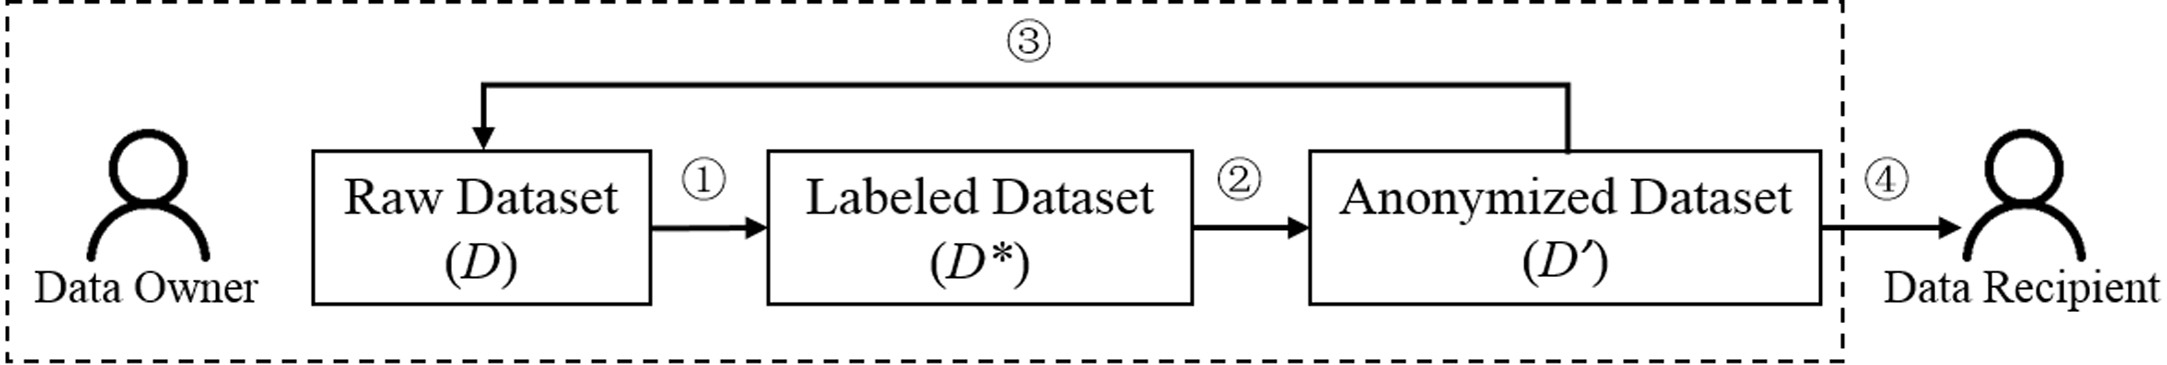
\includegraphics[width=0.5\textwidth,height=0.1\textwidth]{DPHeter.jpg}}
    \caption{Overview of DPHeter.}
    \label{fig1}
\end{figure}

To producing fake data, there are some solutions based on differential privacy. As an extension of previous work, an approach\cite{b7} focusing on the privacy problems of hierarchical Census data casts the problem of privately releasing group size data as a constraint optimization problem and then introduces a two-step mechanism to based on optimization approach and differential privacy: first produce a noisy version of the dataset whose noise if from the variant of the Exponential Mechanism and second restore the feasibility of the constraints while staying as close as possible to the noisy counts which then develops two versions of dynamic-programming and polynomial-time for putting into practice. A decentralized differential privacy scheme\cite{b8} is put forward for protection over one nodes itself and its neighbours through a two-phase work that first collecting the information of each node for making a decision on appropriate noise scale, and second collecting the subgraph count injected with Laplace noise of each node for adjustment in the first step,While PBCN\cite{b9} is proposed to prevent the privacy leakage in social network which consists of four sub algorithms based on the Laplace Mechanism shown in Fig. 2: After Algorithm 1 clustering the nodes in the original social network graph, Algorithm 2 uses the noise to append interference edges aiming at reconstruct the graph; Algorithm 3 also applies the noise from different distribution randomly to all nodes in groups so that the degrees of the nodes in a group may be disturbed; Algorithm 4 is a reconstruction step based on the result of Algorithm 3 and then Algorithm 5 use the differential privacy technique again in particular not to directly append noise to the elements in the graph but uses it as a basis to decide how to append interference to the structure. 
\begin{figure}[htbp]
    \centerline{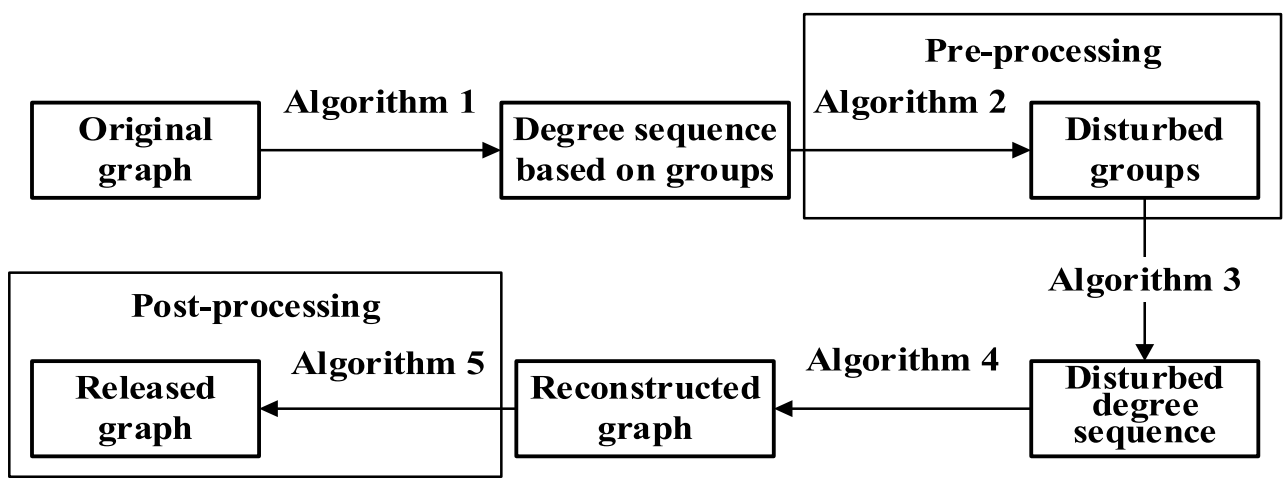
\includegraphics[width=0.5\textwidth,height=0.2\textwidth]{PBCN.png}}
    \caption{Implementation of PBCN.}
    \label{fig2}
\end{figure}\\
DPLT\cite{b10} is a solution which uses the Laplace Mechanism for the publishment of vertically partitioned data based on a latent tree model that the generated latent attributes are able to learn the dependencies of the observed attributes with small noise and then every party participating in the publishment adds noise into both latent attribute pairs of their own local dataset and cross-dataset and the results are aggregated by the curator.

It can be find that differential privacy in dataset protection is always simply to add noise to the data itself. Besides, there is a way to attach differential privacy with generative model to generate fake data might being discussed in later section.

\subsubsection{Training protection}
Despite the complexity of the machine learning models, attackers can still get sensitive information from the models with the prior knowledge of target data, and information disclosure is done by linking the target features with the model outcomes. To handle this problem, several works have been done.

To Regression task, differential pirvacy is helpful in changing the polynomial coefficients to keep the privacy from being revealed. PrivR\cite{b11} combines differential privacy and regression model by dividing the input features into strongly relevant group and weakly relevant group and then calculating the privacy budgets on the basis of the relevance between the input features and the model output which might be used to apply the Laplace Mechanism on the polynomial coefficients of the objective function to realize differential privacy so it can support the model with higher utility by adding variable noise. DPBA\cite{b12} is another work considering the differential privacy in regression analysis that takes the effect of sensitivity among various components in the objective function into account and specifically, it breaks the object function into two parts and then allocate privacy budgets in accordance to the sensitivities of the parts which are computed separately to add noise sampled from the Laplace Mechanism to offer privacy guarantee, and then the model can be optimized by adjusting the allocation of privacy budget and that means the differential privacy will be flexibly applied in regression task. In ADPR\cite{b13} a dynamic privacy allocation mechanism with relevance-based noise imposition is designed where relevance radio, which is computed to qualify how much the input feature contributes differently to the outcome of model, is introduced to adjust the privacy budget of the Laplace Mechanism, so that an adaptive perturbation can be injected into parameters to achieve privacy preserving. A general framework named noise reduction\cite{b14} is proposed which can be applied to a variety of private empirical risk minimization algorithms, by generating a series of hypotheses with a applied policy that separately adding Laplace noise which is gradually increasing and then picking the first satisfying the accuracy demand of empirical risk minimization problem, and what's more, this method is satisfied a looser version of differential privacy proposed at the same time.

It is well known that stochastic gradient descent(SGD) algorithm is the most popular method to update the parameters of neural network whose privacy problem is always arousing public concern. Thus a lot of outstanding works focus on the combination of SGD algorithm and the differential privacy technique. DP-SGD\cite{b15} is the representative one of them where the optimization with differential privacy is divided into two step: at each step of the SGD, first after computing the the gradient of a random sample set, a clip is performed on the $l_2$ norm of each of them and then add noise from the Gauss Mechanism to the result and take the average as the final gradient. The most ingenious feature of DP-SGD is the moments accountant which is proposed to offer more accurate differential privacy for appropriately chosen settings of the noise scale and its detail process is presented: first, compute the log moments of the privacy loss random variable which compose linearly and then use the moments bound together with the standard Markov inequality to obtain the tail bound, that is the privacy loss in the sense of differential privacy. Moments accountant has been widely used for improving the privacy protection ability of models of deep learning so it has to be presented in detailed here. DP-SGD is such a pioneer work that motivates the following work based on it to increase the utility of models through the modify on the structure of neural networks, such as DPNAS employing neural architecture search to automatic model design for privacy training and including three parts based on the design of search space, the DP-aware training method for candidate networks, and the search algorithm: the search space mainly consisting of stacked computation cells, the DP-aware training method which actually is DP-SGD, and the search algorithm based on RNN\cite{b16}, replacing ReLUs with a bounded activation function like the tempered sigmoids\cite{b17} which is reduced the magnitude of a neuron’s activation offering more utility for models training with DP-SDG, GEP\cite{b18} with the help of DP-SGD projecting the private gradients into the anchor subspace which is estimated from the the principal components of non-sensitive data to get low dimensional embeddings and residual expressions and later perturbing the gradient embedding and residual gradient separately with noise from the Gauss Mechanism to achieve differential privacy, by projecting the gradients into subspace which is constructed from an auxiliary public dataset sharing the same distribution with privacy data the PDP-SGD\cite{b19} adding Gauss noise to gradient following DP-SGD which is different from the former one, an approach\cite{b20} for privacy protection in LSTM language models introducing a noised version of the federated averaging algorithm which is based on DP-SGD where two different clip operation is mentioned and the noise from the Gauss Mehcanism is add to the gradients at the cost of increased computation, rather than in decreased utility of models and so on.
\begin{figure}[htbp]
    \centerline{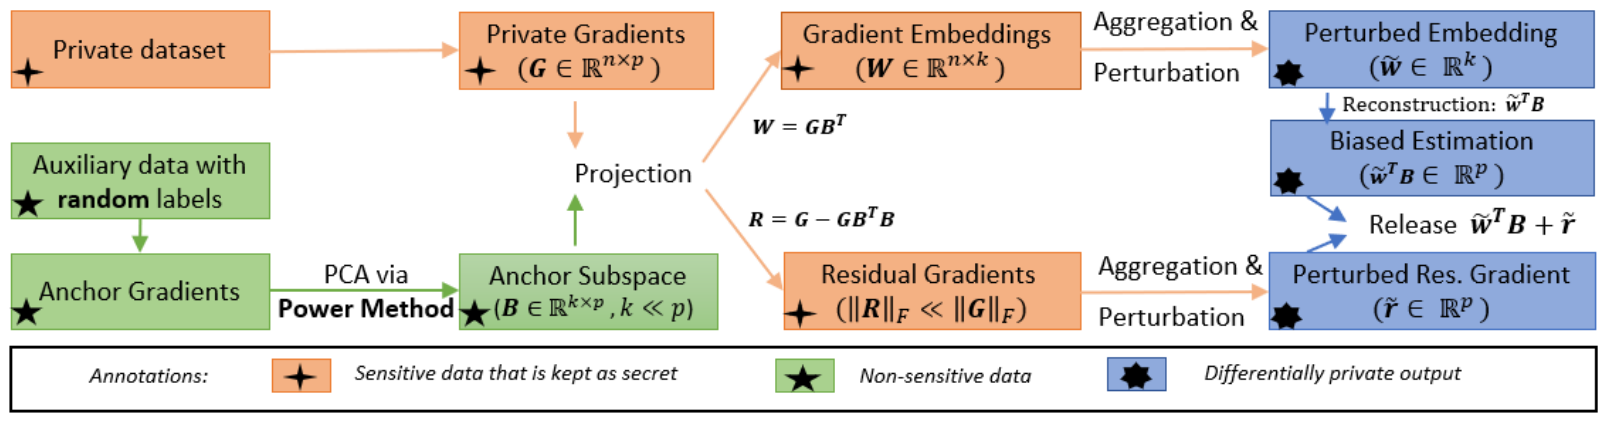
\includegraphics[width=0.5\textwidth,height=0.15\textwidth]{GEP.png}}
    \caption{Implementation of PBCN.}
    \label{fig3}
\end{figure}\\
cpSGD\cite{b21} provides a way to deal with gradient by applying noise from Binomial Mechanism based on stochastic k-level quantization which can achieve nearly the same utility as the Gaussian Mechanism on gradients of client training which are then aggregated in the server end for both communication efficiency and differential privacy in federated setting.

There are also other works focusing on the other steps in neural network training. Adaptive Laplace Mechanism\cite{b22} is designed to perturb affine transformations of neurons and loss functions with Laplace noise and what's more, intentionally add more same kind of noise into features which are less relevant to the model output, and vice-versa.

It is obvious that the differential privacy has had a profound impact in model training that usually acts noise addition to the parameters affecting the models behave to achieve the propose of hiding the privacy information in the model so that bringing more difficult to infer private data to attackers.

\subsubsection{Result protection}
Privacy leakage may occur after model training that from the result the attackers are able to infer the original privacy data even if they do not have direct access to the dataset by simply performing some queries. So there are some excellent works providing subtle ways adopting distributed idea to respond to queries to implement protecting the result itself and it reflects the original intention of differential privacy.

PATE\cite{b23} is a general machine learning strategy that provides differential privacy for training data in a “black-box” manner in classification task, which takes steps shown in Fig. 4 that first privacy dataset is divided into several disjoint subsets for training several teacher models when which reach a strong quorum, this allows PATE to bound privacy costs more strictly, for the majority outcome has overwhelming likelihood, in which case the privacy cost is small whenever this outcome occurs; second, an aggregation operation that all teachers votes on the data is done to gather the prediction and noise sampled from the Laplace Mechanism where take the usage of moment accountant for tightening the privacy bound is added to the result for introducing the ambiguity of differential privacy; third, a student model which learns separately to predict an output using the public dataset and the noisy voting among all of the teachers can not directly access an individual teacher or the underlying data or parameters and moments accountant is used to keep track of the privacy budget throughout the student’s training which is inspired from a native idea that to bound our approach’s privacy loss is to first bound the privacy cost of each label queried by the student, and then use the strong composition theorem to derive the total cost of training the student, and here is a trick to solve the privacy exposure caused by computing moment accountant: the smooth sensitivity of the moments is bound and noise proportional is added to the moments themselves, giving a differential private estimate of the privacy cost. Indeed, the student model is the actual one holding the guarantee of differential privacy, but it is mentioned that the number of teachers in PATE also has effect on the privacy cost that the gap between the top two highest class in the voting of teachers itself increases with the number of teachers, which means having more teachers would lower the privacy cost. 
\begin{figure}[htbp]
    \centerline{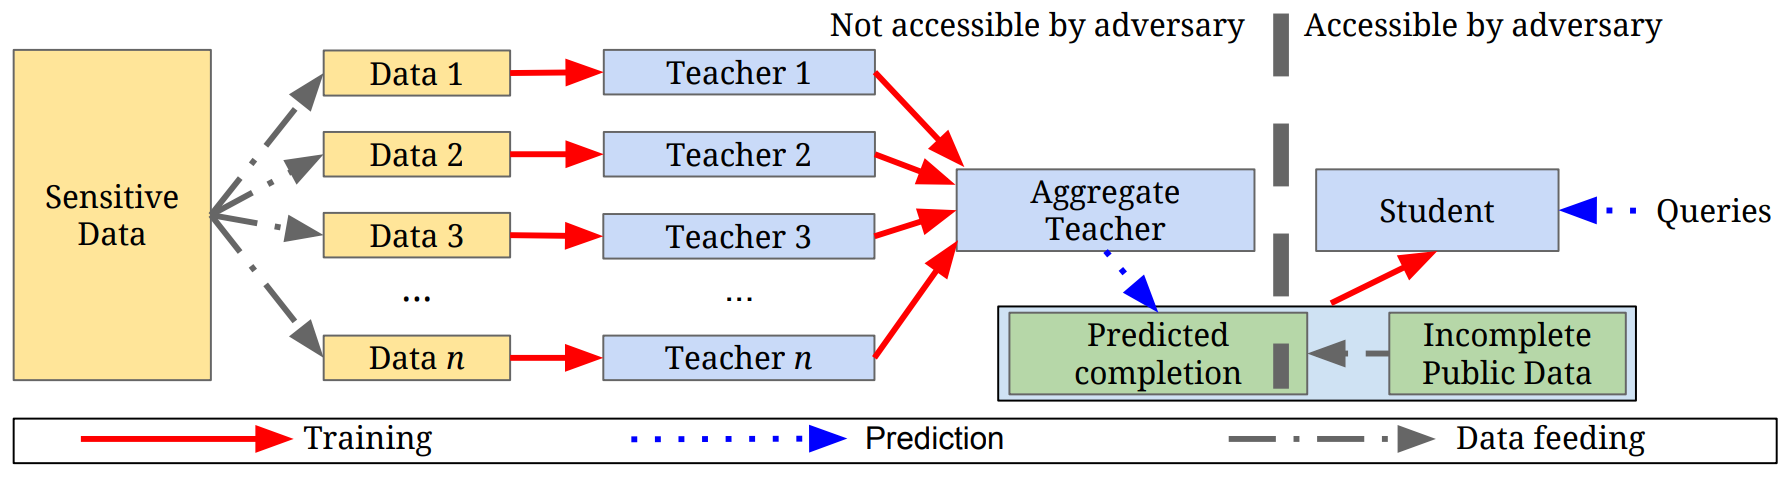
\includegraphics[width=0.5\textwidth,height=0.15\textwidth]{PATE.png}}
    \caption{Overview of PATE.}
    \label{fig4}
\end{figure}\\
Meanwhile a new mechanisms\cite{b24} where teachers and student play the same roles in PATE-G is put forward as an extension of PATE-G which is build on two insights: the chance of teachers' consensus is increased by using more concentrated noise and lacking consensus which means no answer need be given to a student by developing new aggregation for teachers which is more selective and is able to add less noise, allowing PATE to be applied on a larger scale to build more accurate models, in a manner that improves both on PATE’s intuitive privacy-protection due to the teachers’ independent consensus as well as its differential-privacy guarantees: this work adds Gaussian noise with an accompanying privacy analysis in the Rényi differential privacy framework to perform the GNMax mechanism to improve the aggregation of teachers, and this kind of the differential privacy technique not only helps directly improve the aggregation’s utility when the number of classes is large, but also leads to loose privacy bounds; then two aggregation methods that takes into account not only teacher votes on a queried example but possible student predictions on that query which are the Confident-GNMax Aggregator that enables to filter out queries for which teachers do not have a sufficiently strong consensus to avoid answering expensive queries by checking if the plurality vote crosses a threshold where the comparison is done after adding Gaussian noise to enforce privacy, where if queries passing the threshold check, the aggregator proceeds with the usual GNMax mechanism, while if not, the aggregator simply returns nothing and the student discards this example in its training and the Interactive-GNMax Aggregator that discards queries where the student already confidently predicts the same label as the teachers by comparing student predictions to teacher votes for each class where if the difference between them crosses a noisy threshold, the GNMax mechanism is applied while if not, the aggregator reinforces the predicted student label if the student is confident enough and does this without looking at teacher votes again. DPKD\cite{b25} is an extension work of PATE which performs knowledge distillation on teacher models through the same softmax temperature to compute the component probability for predicion containing knowledge about the relative differences between data and modifies the conventional framework by adding noise to prediction of all teacher models before aggregation instead, and the key part of it is shown in Fig. 5. 
\begin{figure}[htbp]
    \centerline{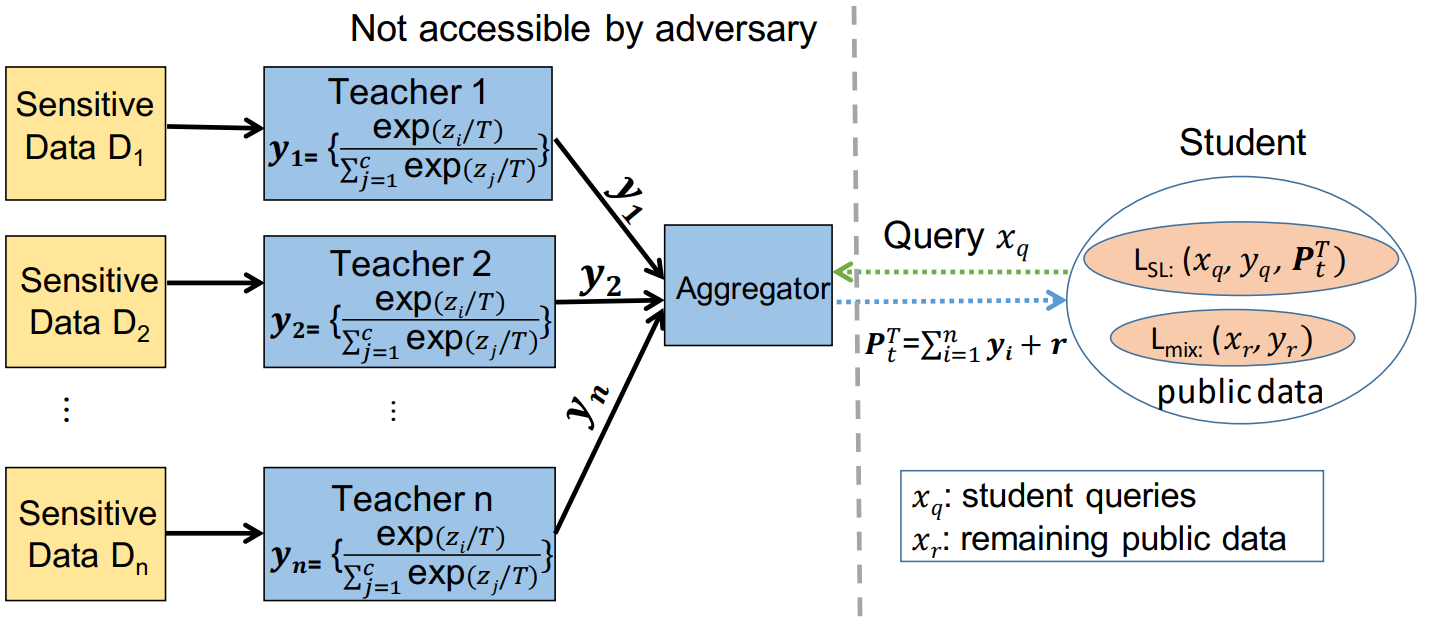
\includegraphics[width=0.5\textwidth,height=0.2\textwidth]{DPKD.png}}
    \caption{The Key of DPKD.}
    \label{fig5}
\end{figure}

Federated learning is one of the most common scenarios for differential privacy protection of results, because the communication between the clients and servers is not so security and in addition, the clients may not will their privacy data exposed to the server. By designing Bayesian differential privacy which allows clients to adjust the privacy budget depending on the data distribution of the datasets with the assumption that all data shares the same distribution, a scheme\cite{b26} performs noise addition to the parameters passing to the server in order to improve service quality. When dealing with the parameters passing to server in alternating direction method of multipliers (ADMM) algorithm a differentially private parameter sharing mechanism\cite{b27} is designed that the Gauss distribution which the noise is from takes a certain proportion of clients into account so that the sum of parameters received by server contains sufficient noise to guarantee differential privacy and keep the error of the sum to be small at the same time combined with a cryptographic construction making the server have a knowledge about global parameters. In an optimization algorithms named Fadam\cite{b28} that that combines the adaptive gradient descent strategy with federated learning, the gradients from clients are normalized and scaled in order to to avoid excessive contribution before noise of the Gauss Mechanism is appended to them based on data characteristics and the global sensitivity. 

Another research interest is to apply the disturbance on the privacy answers themselves. With the assumption that the $L_2$ norm of any column of the queries matrix is bounded from above by some arbitrary constant, an algorithm\cite{b29}  is proposed that adding Gaussian noise to the privacy answer distribution so the queries might getting the wrong answers in probability to solve both non-adaptive and adaptive versions of the problem of estimating a set of linear queries with respect to some unknown distribution under the constraint of local differential privacy. 

Playing the differential privacy techniques on the result is the last defence against the privacy thieves. When faced with the queries, the most approaches proposed is to add noise to what is need to expose and sometimes putting interference to queries itself can be another efficient way.

The differential privacy has been successfully applied in the field of machine learning, where a great amount explorations are going on to embed the privacy preserving into the artificial intelligent service preventing people from the breach of privacy.

\subsection{Variants of Differential Privacy}
Since it was proposed, $(\epsilon, \delta)-differential \quad privacy$ has been widely accepted by academia and industry, and it is always the first option to perform privacy promise in the implement of privacy preserving algorithms. Although compared with the $(\epsilon, 0)-differential \quad privacy$, it permits more flexibility when building modules of differential privacy methods. But it seems not perform well in the composition of differential privacy mechanism. To make up for the shortcoming of $(\epsilon, \delta)-differential \quad privacy$, two new forms of differential privacy are proposed, both of which use Rényi divergence.

\subsubsection{Zero-concentrated Differential Privacy\cite{b30}}
Zero-concentrated differential privacy is based on another work called concentrated differential privacy which is a randomized mechanism whose privacy loss has small mean and is subgaussian. A randomized mechanism is $(\xi, \rho)-zero-concentrated \quad differential \quad privacy$ if it meets the following definition:
\begin{equation}
    D_{\alpha}(M(D)||M(D')) \leq \xi + \rho \alpha,
\end{equation}
where $D$ and $D'$ are neighbouring datasets and $D_{\alpha}(M(D)||M(D'))$ is the $\alpha - R\acute{e}nyi \quad adivergence$ between the distribution of $M(D)$ and $M(D')$ which measures the dissimilarity between them. Rényi divergence can be computed as following:
\begin{equation}
    \begin{split}
        D_{\alpha}(P||Q) &=\frac{1}{\alpha - 1}log(E_{x \sim Q}(\frac{P(x)}{Q(x)})^\alpha)\\
        &=\frac{1}{\alpha - 1}log(E_{x \sim P}(\frac{P(x)}{Q(x)})^{\alpha - 1}).
    \end{split}
\end{equation}
Here $P(\cdot)$ and $Q(\cdot)$ denote the probability density function, and $\alpha \in (0, \infty)$. The same as $(\epsilon, \delta)-differential \quad privacy$, when $\xi = 0$, it is said that $M$ is $\rho-zero-concentrated \quad differential \quad privacy$. When the outputs of $M(D)$ and $M(D')$ are focused, it is easily to come a conclusion that probability of the situation that they are the same is quite higher than others which actually corresponds to a Gaussian distribution with mean $\xi + \rho$ and variance $2\rho$, so it might be difficult to tell where the output comes from. Zero-concentrated differential privacy can be thought to provide guarantees of $(\epsilon, \delta)-differential \quad privacy$: if $M$ provides $\rho-zero-concentrated \quad differential \quad privacy$, then $M$ is $(\rho+2\sqrt{\rho log(1/\delta)}, \delta)-differential \quad privacy$ and if $M$ satisfies $\epsilon-differential \quad privacy$, then it satisfies $(\frac{1}{2}\epsilon^2)-zero-concentrated \quad differential \quad privacy$, while if $M$ satisfies $(\epsilon, \delta)-differential \quad privacy$ looser than the strict form, it may become a little complex that it is $\delta-approximate \quad (\frac{1}{2}\epsilon^2)-zero-concentrated \quad differential \quad privacy$. The definition of $\delta-approximate \quad \rho-zero-concentrated \quad differential \quad privacy$ is given as:
\begin{equation}
    \begin{split}
        D_{\alpha}(M(D)_E||M(D')_{E'}) \leq \xi + \rho \alpha,\\
        D_{\alpha}(M(D')_{E'}||M(D)_E) \leq \xi + \rho \alpha.\\
    \end{split}
\end{equation}
Here $M(D)_E$ means the distribution of $M(D)$ conditioned on the event $E$, and both the probability of event $E$ and $E'$ are $1-\delta$. The feature of privacy post-processing and composability keep in zero-concentrated differential privacy. The composition of two zero-concentrated differential privacy mechanism, one of which is $\rho_1-zero-concentrated \quad differential \quad privacy$ and the other is $\rho_2-zero-concentrated \quad differential \quad privacy$, is $(\rho_1 + \rho_2)-zero-concentrated \quad differential \quad privacy$. But when faced with group privacy, there is a fact that a differential privacy mechanism $M$ following $\rho-zero-concentrated \quad differential \quad privacy$ will guarantees $(k^2\rho)-zero-concentrated \quad differential \quad privacy$ for group of size $k$.

\subsubsection{Rényi Differential Privacy\cite{b31}}
Rényi differential privacy is also based on Rényi divergence, but compared with the definition of zero-concentrated differential privacy shown in $(17)$, the definition of Rényi differential privacy has a change on the right hand of inequality:
\begin{equation}
     D_{\alpha}(M(D)||M(D')) \leq \epsilon.
\end{equation}
If a randomized algorithm follows the above definition, then it might be regarded to meet $(\alpha, \epsilon)-R\acute{e}nyi \quad differential \quad privacy$. By less limitation, Rényi differential privacy allows more accurate numerical analysis for specific task, and it provides a relaxed guarantee as shown:
\begin{equation}
    \begin{split}
        e^{-\epsilon}Pr[M(D') \in S]^{-\alpha \ (\alpha - 1)} &\leq Pr[M(D) \in S]\\
        &\leq e^{\epsilon}Pr[M(D') \in S]^{-\alpha \ (\alpha - 1)}
    \end{split}
\end{equation}
In Rényi differential privacy, the nature of post-processing holds. Besides, it can be used as a block to ompose more complex privacy protection algorithm because of its composability, but it also can not avoid the reduction on privacy protection that if $M_1$ is $(\alpha, \epsilon_1)-R\acute{e}nyi \quad differential \quad privacy$ and $M_2$ is $(\alpha, \epsilon_2)-R\acute{e}nyi \quad differential \quad privacy$, then their composition is $(\alpha, \epsilon_1 + \epsilon_2)-R\acute{e}nyi \quad differential \quad privacy$. In group privacy, a algorithm following $(\alpha, \epsilon)-R\acute{e}nyi \quad differential \quad privacy$ perform as $(\alpha / 2^c, 3^c \epsilon)-R\acute{e}nyi \quad differential \quad privacy$ on the group whose size is $2^c$. Same as zero-concentrated differential privacy, Rényi differential privacy can be treated in form of $(\epsilon, \delta)-differential \quad privacy$: if $M$ is $(\alpha, \epsilon)-R\acute{e}nyi \quad differential \quad privacy$, it also satisfies $(\epsilon + \frac{log 1 \delta}{\alpha - 1}, \delta)-differential privacy$.

From above, it can be seen that Rényi divergence is the generalization form to describe the difference between two distributions as shown in $(18)$, and actually plays an important role in development of differential privacy techniques. So it is intuitively it can also be used for $\epsilon-differential \quad privacy$. Of course, it is true when $\alpha \longrightarrow \infty$, for a randomized mechanism $M$ satisfying $\epsilon-differential \quad privacy$, its its distribution over any two neighbouring dataset $D$ and $D'$ is meet the below:
\begin{equation}
    D_{\infty}(M(D)||M(D')) \leq \epsilon,
\end{equation}
which is the other representation of the definition of $\epsilon-differential \quad privacy$. 

For further work on differential privacy, it is foreseeable that some more differential privacy may appear for different demands of privacy preserving according to given parameter variation.

\section{Generative Models}
It is necessary to learn about the principles of generative models before having a acquaintance with their combination with the differential privacy. In this work, Generative Adversarial Network and Variational Autoencoder will be introduced in detail for their popularity in the field of generative models.

\subsection{Generative Adversarial Network\cite{b32}}
Generative Adversarial Network(GAN) is one of the most popular models in the field of deep learning and since its proposal, it has quickly become a hot research topic.

In the framework of GAN which corresponds to a mini-max two-player game, two models defined by multilayer perceptrons are simultaneously trained with backpropagation: a generative model $G$ that captures the data distribution, and a discriminative model $D$ that estimates the probability that a sample came from the training data rather than $G$. The training procedure for $G$ is to maximize the probability of $D$ making a mistake and when the data distribution generated by $G$ is identified by $D$ with a probability equal to $\frac{1}{2}$, the whole system achieves a optimal state.

In other words, $D$ and $G$ play the following two-player mini-max game with value function $V(G, D)$:
\begin{equation}
    \begin{split}
        min_Gmax_DV(G, D) &= E_{x \sim p_{data}(x)}[logD(x)]\\ 
        &+ E_{z \sim p_{z}(z)}[log(1-D(G(z)))],
    \end{split}
\end{equation}
where $x$ denotes the real data and $z$ denotes the noise data which often obeys the Gauss distribution. $p_data(\cdot)$ represents the probability distribution of data. $D(x)$ computes the probability that $x$ comes from the data rather than $G(z)$ which is a mapping from noise to data. From the perspective of $D$, it is trained to maximize the probability of assigning the correct label to both training data and samples generated by $G$, while from the perspective of $G$, it is trained to minimize the probability. It is noted that the training frequencies of $D$ and $G$ are different that a training period consists of $k$ times for updating $D$ and one time for $G$.

For any given $G$ fixed, the optimal $D$ is satisfied the following condition :
\begin{equation}
    D^*_G(x)=\frac{p_{data}(x)}{p_{data}(x) + p_{g}(x)},
\end{equation}
where $ p_{g}$ is defined as a probability distribution of of the samples $G(z)$ and then (23) can be reformulated as:
\begin{equation}
    \begin{split}
        C(G) &= max_DV(G, D)\\
            &= E_{x \sim p_{data}}[logD^*_G(x)] + E_{z \sim p_{z}}[log(1-D^*_G(G(z)))]\\
            &= E_{x \sim p_{data}}log[\frac{p_{data}(x)}{p_{data}(x) + p_{g}(x)}]\\
            &+ E_{x \sim p_{g}}log(1-\frac{p_{g}(x)}{p_{data}(x) + p_{g}(x)}).\\
            &= -log(4) +KL(p_{data}||\frac{p_{data}+p_g}{2})+KL(p_{g}||\frac{p_{data}+p_g}{2})\\
            &= -log(4)+2\cdot JSD(p_{data}||g_g),
    \end{split}
\end{equation}
where $KL(\cdot||\cdot)$ is the Kullback–Leibler divergence, and $JSD(\cdot||\cdot)$ is Jensen–Shannon divergence. So it can be seen that when $p_{data} = p_g$, $C(G)$ achieves the minimum, i.e. the GAN reach its peak of generation ability.

\subsection{Variational Autoencoder\cite{b33}}
Variational Autoencoder(VAE) is another popular work of generative models that is considered as a useful tool widely applied for generation in many fields.

The main idea of VAE is that by encoding the input to obtain a latent representation vectors, the model then decodes the latent vectors to generate the output result similar to the input one. In its framework, the encoder $q(z|x)$ captures the probability distribution of the latent representation $z$ when input $x$ is given, and the decoder $p(x|z)$ captures the probability distribution of $x$ with the given latent $z$. 

The training procedure of the system is to maximize $p(x)$, which is the probability of input $x$:
\begin{equation}
    max \sum_x log(p(x)) = max \sum_x log(\int_zp(x|z)p(z)dz),
\end{equation}
where $p(z)$ denotes the probability of $z$ sampled randomly from a distribution. It is noted that the encoder ought to be introduced, so the $logP(x)$ should be reformulate as:
\begin{equation}
    \begin{split}
        log(p(x)) &= \int_zq(z|x)log(p(x))dz\\
        &= \int_zq(z|x)log(\frac{p(z,x)}{q(z|x)}dz) + \int_zq(z|x)log(\frac{q(x|z)}{p(z|x)}dz)\\
        &= L_b + KL(q(x|z)||p(z|x)),
    \end{split}
\end{equation}
and here $L_b$ can be rewritten as:
\begin{equation}
    \begin{split}
        L_b &= \int_zq(z|x)log(\frac{p(z,x)}{q(z|x)}dz)\\
        &= \int_zq(z|x)log(\frac{p(z)}{q(z|x)}dz) + \int_zq(z|x)log(p(x|z)dz)\\
        &=-KL(q(z|x)||p(z)) + \int_zq(z|x)log(p(x|z)dz)
    \end{split}
\end{equation}
From $(27)$, it can be seen that to maximize $\sum_x logp(x)$ needs to increase $L_b$ that means decreasing $KL(q(z|x)||p(z))$ in $(28)$, i.e. let encoder $q(z|x)$ approach to $p(z)$ and increasing decoder $p(x|z)$. As a result, the loss function of VAE can be defined as following:
\begin{equation}
    \begin{split}
        L &= -KL(q(z|x)||p(z)) + \int_zq(z|x)log(p(x|z)dz)\\
        &= \frac{1}{2} \sum_{j=1}^n (1+exp(log((\sigma_j^i)^2)-(\mu_j^i)^2-(\sigma_j^i)^2)\\
        &+\frac{1}{L}log(p(x^i|z^{i,l})),
    \end{split}
\end{equation}
where $x^i$ means $i-th$ data and $z^{i,l}$ means the latent representation encoded by encoder $q(z|x^i)$ which produces $\sigma^i$ and $\mu^i$ with the variational approximate posterior being a multivariate Gaussian with a diagonal covariance structure:
\begin{equation}
    log(q(z|x^i))= log(N(z;\mu^i,\sigma^{2i}I)
\end{equation}
In practical, the encoder and decoder in VAE is trained simultaneously.

It ought to be known that the generative models themselves can be regarded as a tool to perform privacy preserving but the generated data still reveals the structure of models from which the privacy data can be interfered. In fact, some researches put great efforts on combining the differential and the generative models.

\section{Differential Privacy in Generative Models}
According to the type of generative models, works on GAN and VAE combined with the differential privacy will be introduced separately.

\subsection{Generative Adversarial Network}
GAN is the most commonly used in combining the differential privacy and the generative models.

PATE-G\cite{b23}, a semi-supervised learning with GANs, is the first successful model used PATE by modifying the discriminator of GAN that only student is discriminator while teachers are regarded as an extra parts to improve the student and both student and teachers are extended from a binary classifier which can only tell the data come from real dataset or the generated samples to a multi-class classifier which can identify the data from one of the classes of data samples or the class for generated samples to make full use of the entire data available to the student. In PATE-G, the generator is trained with the loss of student discriminator. However, PATE-G still works under the situation that the output is not distinctly defined by the input features.  PATE-GAN\cite{b34} modifies the basic PATE framework whose noisy aggregation results in a classifier not differentiable with respect to the parameters of the generator to make it more suitable for GAN where differently from PATE-G both student and teachers are discriminators and teachers are trained separately with their own subdataset and the fake data, but the student is trained only with the teacher-labelled generated data some of which is generated fake data and the rest of which is realistic and can be generated by initializing the parameters of the generator randomly using Xavier initialization. To balance the number of teachers and the noise scale, the numbers of generated sample and real records is take the usage of the dimension of the input space which might lead to the low utility of a single teacher but high utility of the resulting classifier actually by aggregating and moreover means the tighter differential privacy guarantees, so that a lower privacy cost is attributed to accessing the noisy aggregation of the teachers when the teachers have a stronger consensus with the intuition being that when the teachers have a strong consensus, a single teacher has a much lower influence on the output than when the votes are close. These changes enable PATE-GAN to tightly bound the influence of any individual sample generation of the model, resulting in the tight differential privacy guarantees and thus an improved performance over models with the same guarantees. The workflow of PATE-GAN can be seen in Fig. 6.
\begin{figure}[htbp]
    \centerline{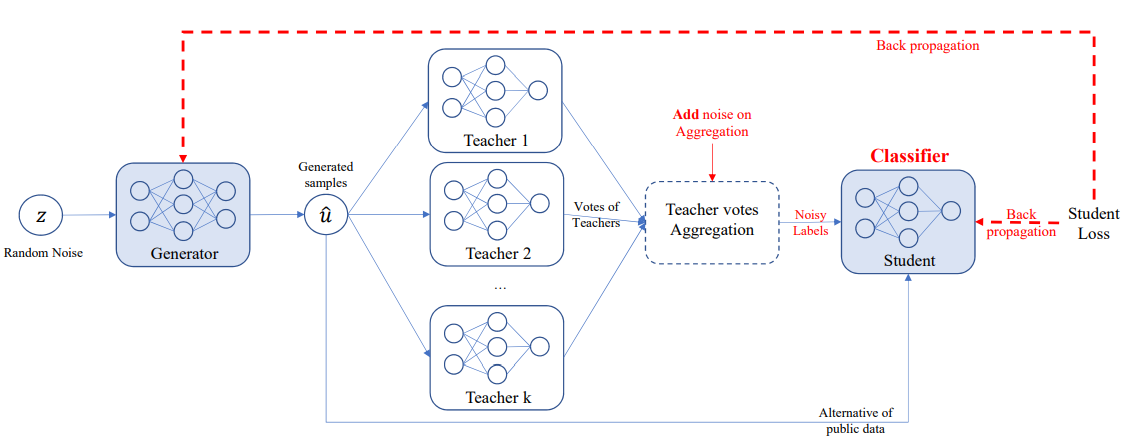
\includegraphics[width=0.5\textwidth,height=0.2\textwidth]{PATE-GAN.png}}
    \caption{The workflow of PATE-GAN.}
    \label{fig6}
\end{figure}\\
As structure shown in Fig. 7, G-PATE\cite{b35} is another example to use PATE in GAN specially treating the generator as the student and the discriminators as the teachers yet, with the proposal of new aggregation that due to random projection and gradient discretization makes this work able to deal with high-dimensional gradient vectors leading to a result of significant improvement on the use of privacy budgets and of the increase in model scalability, that enables gradient aggregator to add noise in the information flow from the teacher discriminators to the student generator to ensure differential privacy by updating the student generator in three steps: fisrt, teacher discriminators generate the backpropagated gradients for each record produced by the student generator and to solve the problem that the privacy information can not be obtained by the student, the backpropagated gradients  are calculated on the fake record by ascending its gradients on the loss of the discriminator which can be viewed as an adversarial perturbation on the fake data that would cause the discriminator’s loss on it to increase; second, the gradient aggregator named DPGradAgg takes the gradients from all teacher models and generates a differential private aggregation of them that is combining the gradient discretization where first a histogram is created and each element is mapped to the midpoint of the bin it belongs to and then teacher discriminators vote for these bins associated with the elements in their gradient vector and last for each dimension, the bin with most votes is computed using the Confident-GNMax Aggregator to convert gradient aggregation into a voting problem and to get the noisy aggregation of teachers’ votes and random projection where a random projection matrix with each component randomly drawn from a Gaussian distribution is generated which then is used to project the gradient vector into a lower dimensional space and after the aggregation, the aggregated gradient vector is projected back to its original dimensions to reduce the dimension of vectors on which the aggregation is performed which is beneficial to privacy protection for maximizing the amount of information a student generator can get from a single query and making it possible for G-PATE to retain reasonable utility even on high dimensional data.; third, given the gradient vector where the teacher discriminators have higher loss on the perturbed fake record compared to the original fake record, the student generator updates its weights based on the privately aggregated gradients that the student generator learns to improve its fake records by minimizing the mean squared error between its output and the perturbed fake record. Therefore, G- PATE uses privacy budget more efficiently and better approximates the real data distribution to ensure high data utility.
\begin{figure}[htbp]
    \centerline{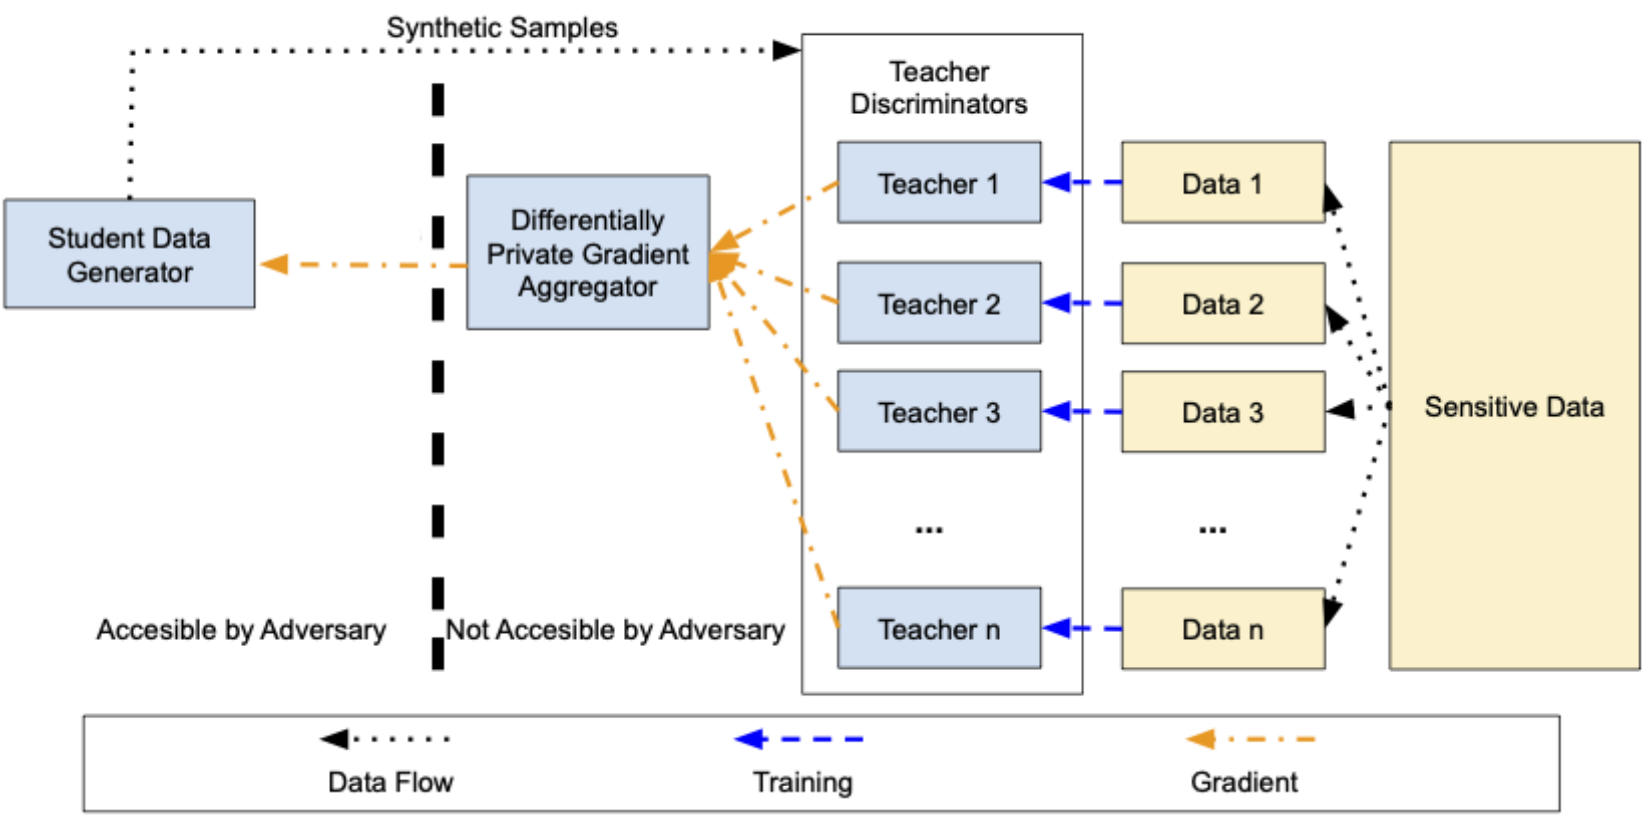
\includegraphics[width=0.4\textwidth,height=0.2\textwidth]{G-PATE.png}}
    \caption{The Structure of G-PATE.}
    \label{fig7}
\end{figure}

The method to use differential privacy mechanism that is to influence gradient is another mainstream to provide the privacy guarantee, and most works adopting the method bring their own measure to deal with the gradients of discriminator in the GAN. With the development of GAN, the differential privacy is also extended to combined with different variant of GAN. An approach\cite{b36} tries to apply DP-SGD in training GAN whose loss is based on the Wasserstein distance to provide privacy protection for time aware continuous or discrete data that is introduced to gradients of discriminator is clipped and the Gauss noise is added to the them when updating the discriminator according to the privacy budget computed with moment accountant where the parameter of gradient clip is dealt with a clipping decay mechanism that allows to clip the suitable amount at each step which performs a constrain on the noise. GANobfuscator\cite{b37}, whose framework can is presented in Fig. 8, is a differential private GAN to mitigate information leakage that applies a combination of carefully designed noise and gradient pruning and adopts the Wasserstein distance as an approximation of the distance between probability distributions, which is a more reasonable metric than JS divergence in GAN. When updating the discriminator, the gradient of it is first pruned by injecting the designed noise to ensure that the sensitivity is bounded and then the random noise sampled from the Gauss Mechanism is only here added to the gradient to enforce differential privacy where moment accountant is used to trace the privacy loss for it has direct access to the sensitive information and often features a simpler architecture and a smaller number of parameters, which make it possible to tightly estimate the privacy loss. After that, the pruning is done again to guarantee the $Lipschitz$ property of parameters of discriminator to bound the gradient from each data. The pruning bound ought to be treated carefully for its influence on the sensitive of privacy protection so that constantly monitoring the magnitudes of the gradients before and during the training is performed, as well as adaptively set the pruning bounds based on the average magnitudes. Specifically, with the assumption that besides the private data to train the model, there is an access to a small amount of public data which is available in many settings. So during each training step, a batch of examples are randomly sampled from public data, and the pruning bound of each parameter is set as the average gradient norm with respect to this batch. During the whole training procedure, an optimization algorithm that can adaptively adjust the learning rate according to the magnitude of gradients is applied then to updating the generator and the discriminator. And the parameters of the generator keep the differential privacy of sampled data through those of the discriminator, So the gradients in GANobfuscator can be bounded to avoid unnecessary distortion which not only keeps the loss function with but also provides a sufficient privacy guarantee. With designed framework, GANobfuscator can achieve the task of the generator in GANobfuscator to output a sanitized version of the public data with the privacy constraint and that of the discriminator to learn the private variables from the sanitized data. It is noted that the privacy loss of GANobfuscator is irrelevant to the amount of generated data.
\begin{figure}[htbp]
    \centerline{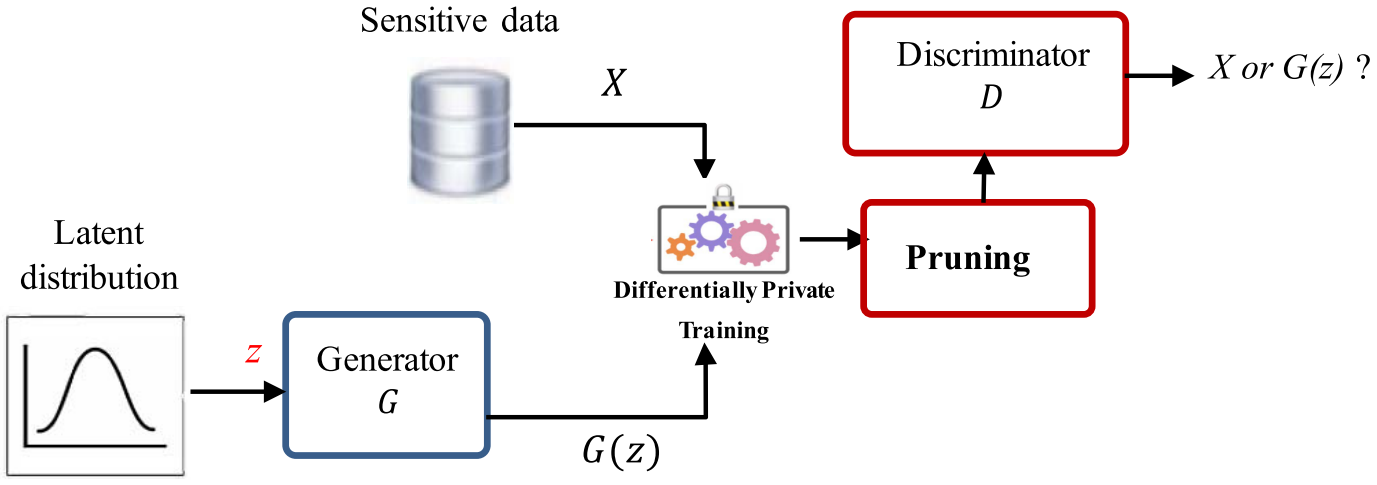
\includegraphics[width=0.5\textwidth,height=0.15\textwidth]{GANobfuscator.png}}
    \caption{The Framework of GANobfuscator.}
    \label{fig8}
\end{figure}\\
DP-CGAN\cite{b38} performs the differential privacy guarantee on the CGAN, the variant of GAN, for generating specific fake data with extra conditions provided which is based on a new clipping and perturbation strategy: by treating the real and the fake data separately, the per-example gradients of the discriminator loss is computed on both of them, and then the per-example gradients are also clipped separately. After the sum of two set of gradients are perturbed with the Gauss noise where RDP accountant based on the Rényi differential privacy used to follow the comsumed privacy budget to provide a tighter bound for privacy loss in comparison with moment accountant works for, the average over all of the perturbed clipped per-example gradients is taken in the batch and final gradients is applied in training the discriminator. It process of updating discriminator is similar to DP-SGD. The differential privacy is also applied to Triple-GAN where a role of classifier is introduced to highlight conditional generation which plays a role of differential privacy identifier\cite{b39} which produces labels for given data that sampled from true data distribution by examining the data through differential private mechanisms that divides streaming data into multiple time slots which are processed respectively where the generated data are required to not only can be identified as differential private-preserving data and also be the adjacent to the generated data that passed the test from the differential privacy identifier at the last time unit under continual observation according to the definition of the differential privacy and pan-privacy. GAN-DP\cite{b40} is also based on the CGAN which takes Wasserstein-1 as the distance distribution measurement to achieve better performance, where two confrontations are gaming simultaneously: the game between the generator that only produces random noise injected into the raw data later rather than the data itself to achieve the differential privacy with high data utility measured by the root mean square error of the value of generated noise and the discriminator; the game between the differential privacy identifier which is leveraged to identify if synthetic data complying with differential privacy framework and the discriminator where the synthetic data cannot be identified by the discriminator while it is keeping differential private. During the training procedure, together with labels representing the privacy data or the input of generator, the differential-private features is compelled to be mapped to associated label as an input of generator. And the optimization targets of three components are descried that for discriminator is the minimization of the difference between generated data and the label itself gives and maximization of that between real data and the label itself gives with a weight parameter; for generator is the minimization of the difference between the generated data and the label given by identifier and that given by discriminator with a weight parameter to indicate how much it relies on the input features;  for identifier is the minimization of the differece between the privacy label and the label itself gives. GAN-DP helps to guide the learning process to generate differential private samples based on the input features rather than only focusing on learning the distribution. It is noted that GAN-DP can be regarded as a GAN driven noise generation mechanism meets the conditions of differential privacy.

Similar to G-PATE, only the generator is trained with differential privacy guarantee in GS-WGAN\cite{b41}, whose approach outline is shown in Fig. 9, by sanitizing gradients that the generator received from the discriminator where it is able to distort gradient information more precisely thereby enabling training deeper models which generate more informative high-dimensional samples that the gradient steps is performed by selectively applying the sanitization mechanism only to the corresponding subset of parameters the scope of which the chain rule is exploited to further narrow in addition, so the  discriminator will be trained more reliably and besides, when doing clipping gradients, by adding the Wasserstein-1 metric which allows to derive a fixed and bounded sensitivity to the loss function of discriminator, its function is $1-Lipschitz continuous$ so the optimal discriminator has a gradient norm being $1$ almost everywhere theoretically, so that the bounded gradients with norms close to 1 is generated by construction which leads to significantly less information destruction when clipping using the sanitization mechanism. For further reduction on the privacy cost during training, GS-WGAN attempts a random mechanism that the whole dataset is subsampled into different subsets and then multiple discriminators is trained independently on each subset and at each training step, the generator randomly queries one discriminator while the selected discriminator updates its parameters on the generated data and its associated subsampled dataset. And moreover, GS-WGAN is naturally allowed for training GANs in both centralized and federated data scenarios where the discriminators are retained at each client and the  sanitized gradients of the samples are transferred to the untrusted server for the generator upadating in GS-WGAN.
\begin{figure}[htbp]
    \centerline{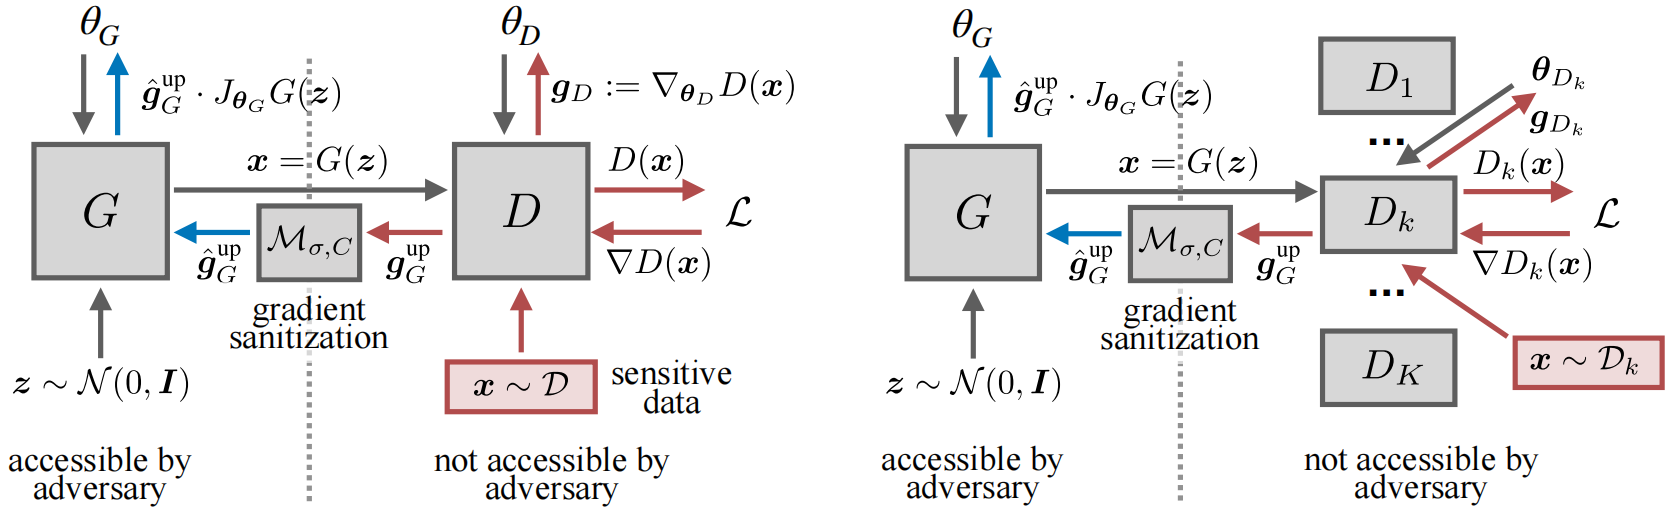
\includegraphics[width=0.5\textwidth,height=0.15\textwidth]{GS-WGAN.png}}
    \caption{Approach Outline of GS-WGAN: left for centralized and the right for federated scenarios.}
    \label{fig9}
\end{figure}\\
Different from GS-WGAN, DP federate GAN\cite{b42} is proposed to adapt GAN training in federated setting by using the DP-FedAvg algorithm that sanitizes gradients of the discriminator in a similar way to DP-SGD which are shared between the clients and the trusted server and of which the unprocessed information is accumulated at the server before being sanitized and the generator is updated via a traditional gradient update without real data at the coordinating server. Local differential privacy also plays an important role in data collection of federated learning, so its combination with GAN attracts some interests as well. A naive solution\cite{b43} whose workflow is shown in Fig. 10 is provided that before the generated data sent to the sever, it is transferred to the discriminator model which is a logistic regression and multi-layer perceptron classifier together with the real dataset to assess whether the generated fake dataset was guaranteed to local differential privacy. If it is satisfied, the generated data will be sent to the server, in contrast, updating the generator model and the discriminator model at the same time according to the backpropagation where the gradients are updated following DP-SGD that is clipped first and perturbed by the addition of Gauss Noise and the moment accountant is taken the advantage of to trace the privacy loss during the optimization process.
\begin{figure}[htbp]
    \centerline{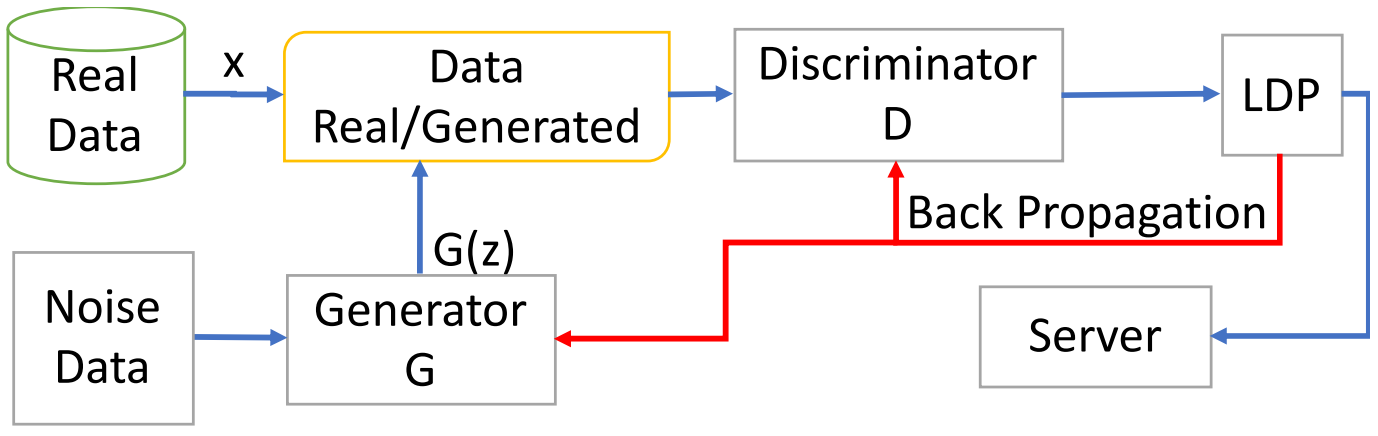
\includegraphics[width=0.5\textwidth,height=0.15\textwidth]{The Workflow of GAN for Local Differential Privacy.png}}
    \caption{The Workflow of GAN for Local Differential Privacy.}
    \label{fig10}
\end{figure}

Another GAN work based on the Rényi differential privacy is proposed in RARIEA\cite{b44} which is a market framework specially designed for trading private data generator, with the help of the Gauss Mechanism where $L-Lipschitz$ and $\beta-smoothness$ to bound the privacy budget of the Rényi differential privacy on data to add noise not only to the parameters of the discriminator but the gradient of the generated data and the privacy data passed from the discriminator to the generator when training. What's more, the differential privacy here is also used as a tool to quantify the privacy loss. 

There is another way to apply the differential privacy and GAN that generates the embeddings of data so that the noise can be attached to the data itself to guarantee the privacy promise. A solution\cite{b45} to address the task of facial identity obfuscation is based on the application of the differential privacy to image encodings in a GAN that applies the framework of the differential privacy to a novel extension of AttGAN where the encodings of the images which are first transformed with PCA that provides obfuscated representations are regarded as vectors so that the generalized privacy guarantee for images can be written using a distance function which is noted to be $L_1$ measure with the distance between each pair where the elements scaled to the range $[0, 1]$ under the maximum and minimum of the elements in corresponding positions in all vectors and the overall vector distance similarly scaled will be gotten, and then the differential privacy guarantee can be achieved by independently adding Laplace noise to each element of the vector such that the element at the corresponding position uses a distribution with a scaled parameter, too, where the addition of noise should be noted that is also causes the loss function of generator of GAN for maintaining the basic characteristics of fake data from the real face images, and after that the encodings might be recovered to a representation in its original basis so can be processed as usual to generate the output images. 

\subsection{Variational Autoencoder}
Compared with GAN, the differential privacy is a relatively new technique combined with VAE.

One thought to perform the differential privacy in VAE is to modify the the distribution of the latent representation. A solution\cite{b46} is proposed to tackle anonymization of textual data by the proposal of end-to-end differential private VAE where it is noted that the encoder and the decoder here are both models based on RNN and GRUs and the loss of the entire model is reconstruction loss of building the similar data to the input and the KL loss indicated the difference between the distribution of real privacy data and the latent representation which works at an abstract level by perturbing the latent vectors that provides a global summary of the input texts that the probabilistic encoder is constrained to facilitate differential private latent sampling by using a continuous mean bound in the latent space named vector-valued radial hyperbolic tangent map to enforce the vector $\mu$ inside a unit ball about the origin where the operation of resizing the co-domain often occurs later to shrink latent space leading to an approximate posterior which is differential privacy and besides, to keep the differential privacy from the unbalance between the standard deviations of two inputs causing the ratio of probabilities leakage the privacy feature, the standard deviation is defined as a specify global parameter that is independent of the input rather than the function defined by the encoder. So the noisy latent representations serve as global blueprint for the decoder and achieve the local Rényi differential privacy at the same time. The approach with designed VAE based on the differential privacy can be regarded as complementary since it protects the data during inference. As shown in Fig. 11, VAE is also used as a tool to build the recommendation system  and here DP-SGD also plays a role to provide the guarantee of the differential privacy\cite{b47}. In this work, when generating the user-level priors based on the different users' metadata represented with public pre-trained word embeddings instead of the standard Gaussian distribution for sampling the latent vector to train VAE, the user-specified noise sampled from the Gauss Mechanism is added into the mean–variance pairs which are used to estimate them for differential privacy protection, and then during the training process of model where DP-SGD works, the gradients of each sample of each user is clipped with a optimal clipping bound which is obtained by a recursive algorithm where an objective function is defined to minimize the expected error of actual gradients and estimated ones to pick the minimum from the gradients list of each user sorted in the increasing order, and then the Gaussian noise is added again into the average of the clipped gradients accordingly for each user, finally the average gradients of all users is computed to carry out the update for the gradients for the model, so that can avoids a significant decline in recommendation performance caused by excessive privacy guarantee and the user-level differential privacy will be applied which allows each user to specify its privacy budget for user privacy protection. Beacause of the above two steps, this work can achieve high recommendation precision while maintaining a reasonable privacy guarantee. 
\begin{figure}[htbp]
    \centerline{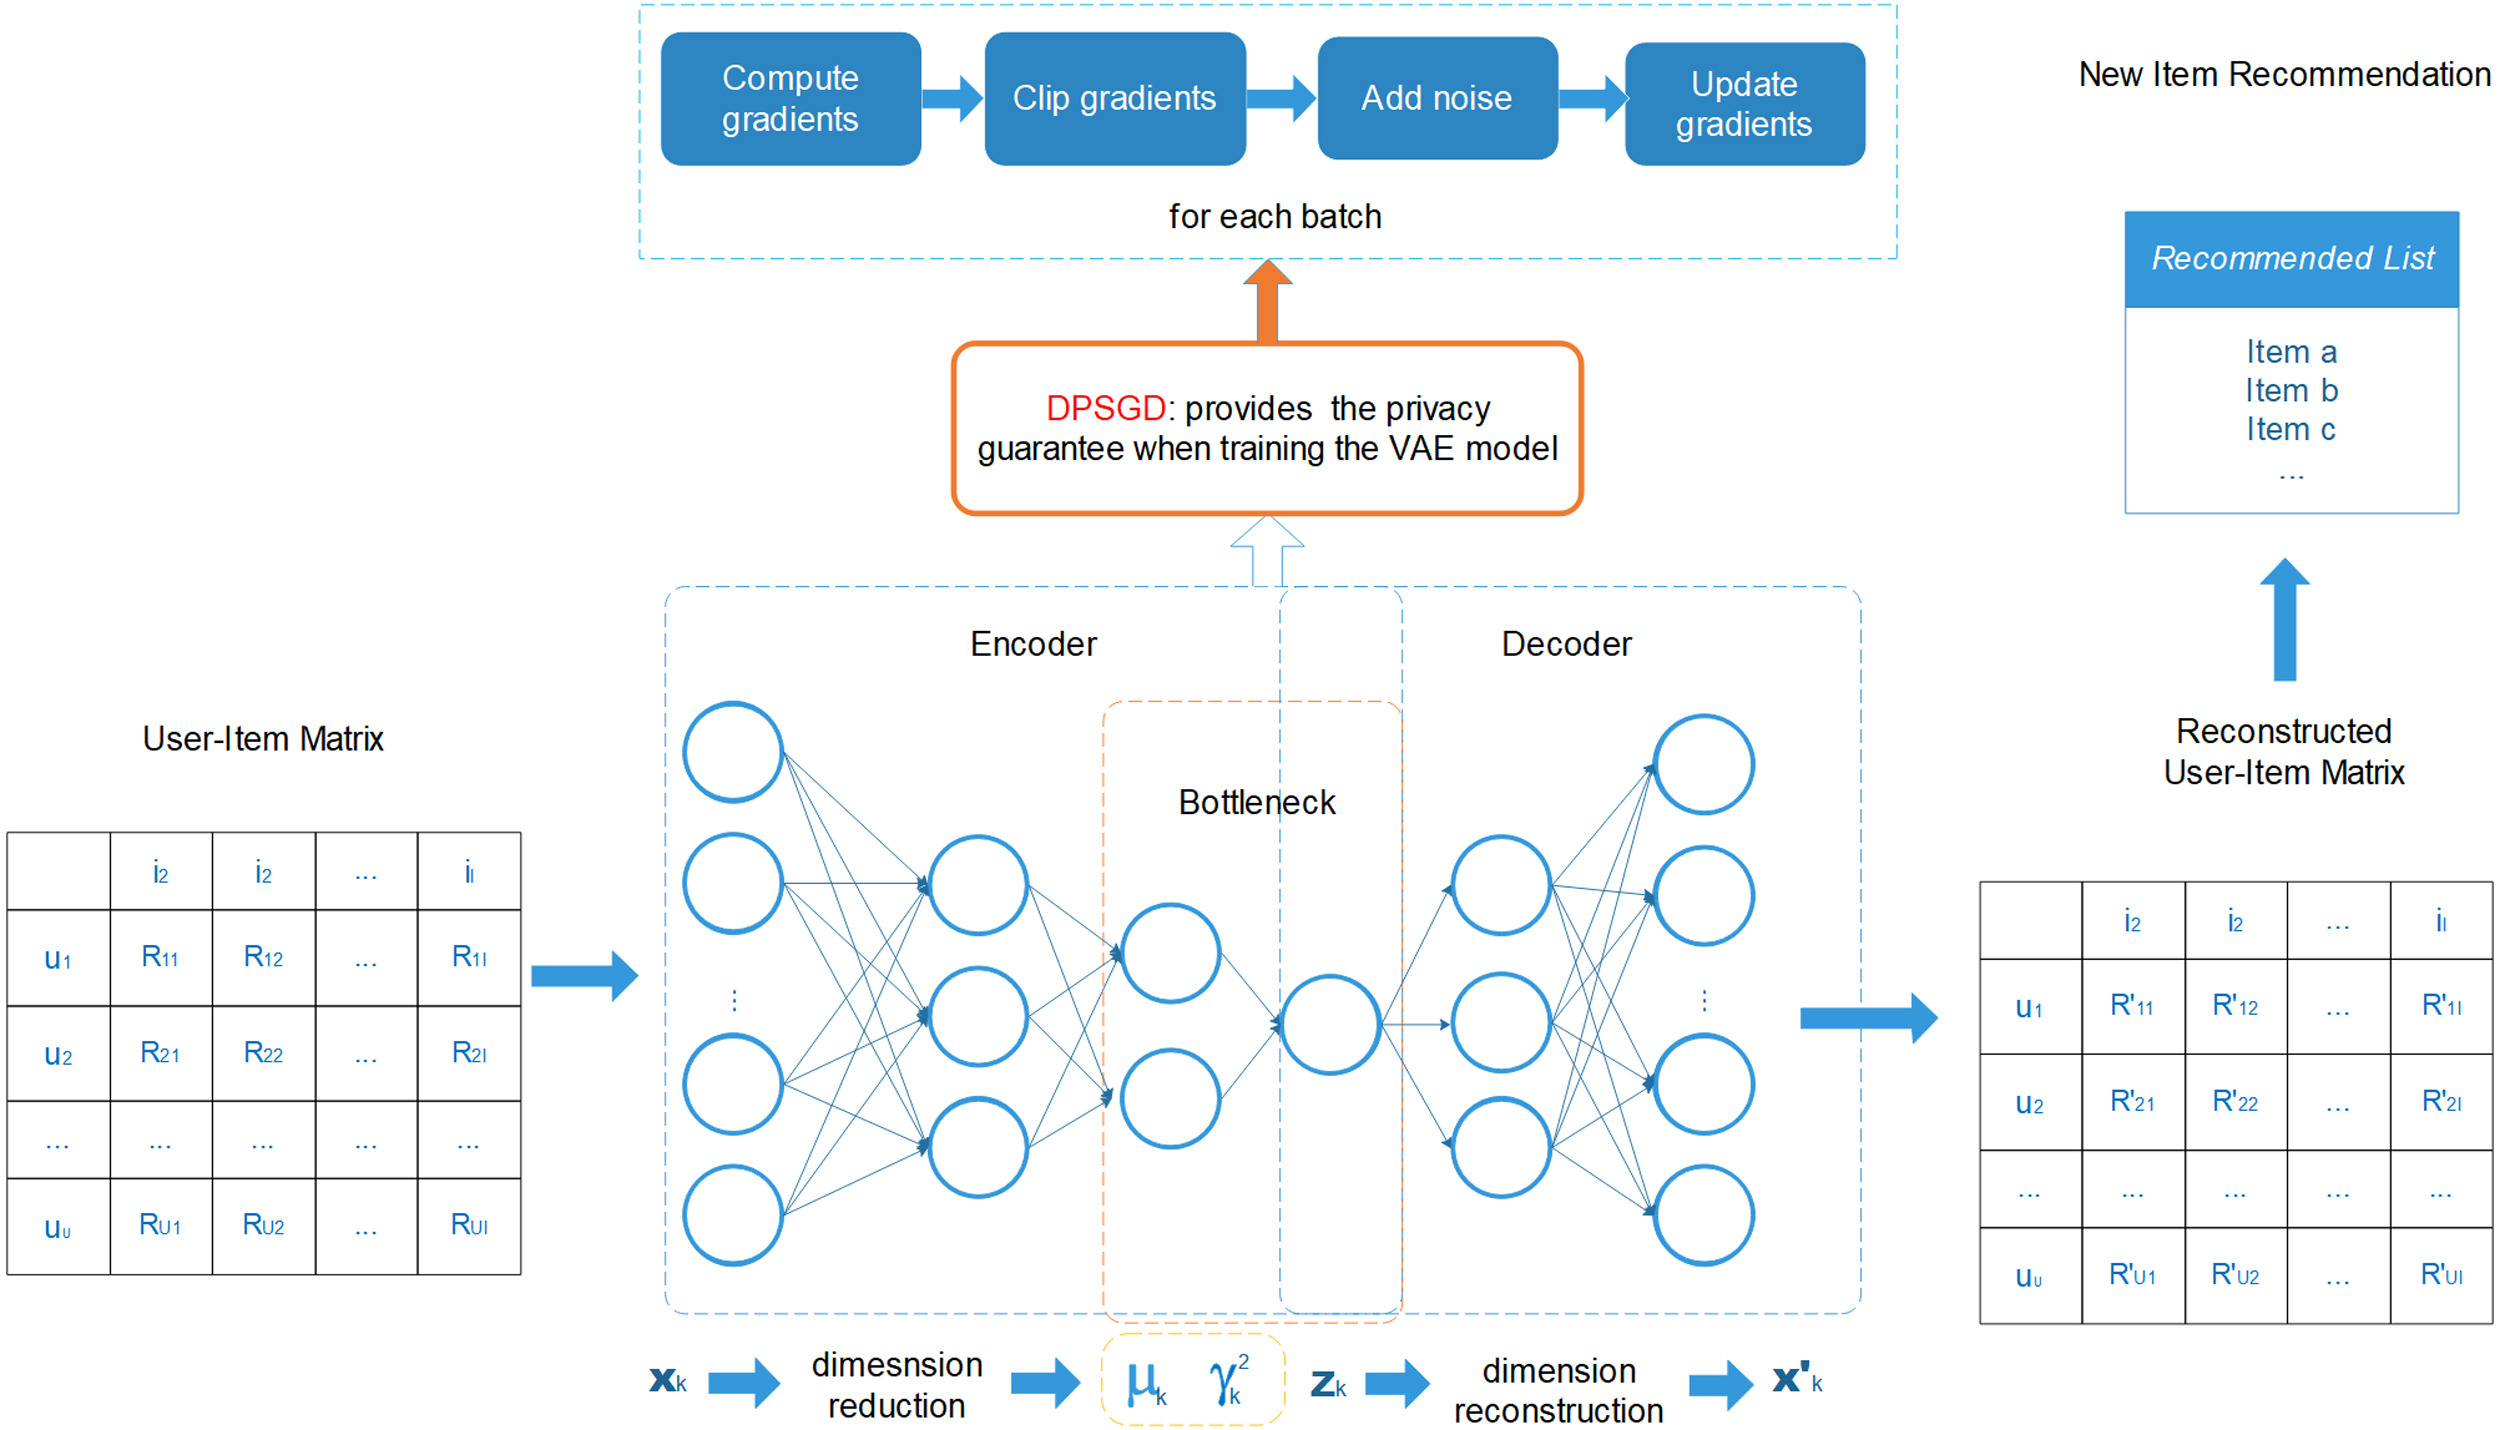
\includegraphics[width=0.5\textwidth,height=0.25\textwidth]{Recommendation System based on DP VAE.jpg}}
    \caption{Recommendation System based on DP VAE.}
    \label{fig11}
\end{figure}\\
In GP-GM\cite{b48} shown in Fig. 12, a differential privacy clustering algorithm combining kernel k-means with random Fourier features is used first to transform the data into low-dimensional representations and then all the feature vectors are clipped with the threshold set to the average norm of them before clustering occurs where different Gaussian noise the scale of which is determined by the $L_2-sensitivity$ of the cluster size and the sum of norms within each cluster is added to the size of all clusters and the sum of all cluster members in each cluster leading to the noisy cluster centers to perform the differential privacy. After each cluster is given to separate VAEs, they are trained with DP-SGD improved with an adaptive selection of clipping threshold which leads to a less noise used to perturb the gradient updates to privacy protection that a random subset of the given cluster is picked for gradients update and the clipping threshold is decided in the same way in clustering that the norm of all samples is computed then the domain of them is discretized by dividing uniformly according to the value to form several gradient groups whose size is counted and the Gaussian noise is added into resulting the maximum of them be the final clipping threshold. 
\begin{figure}[htbp]
    \centerline{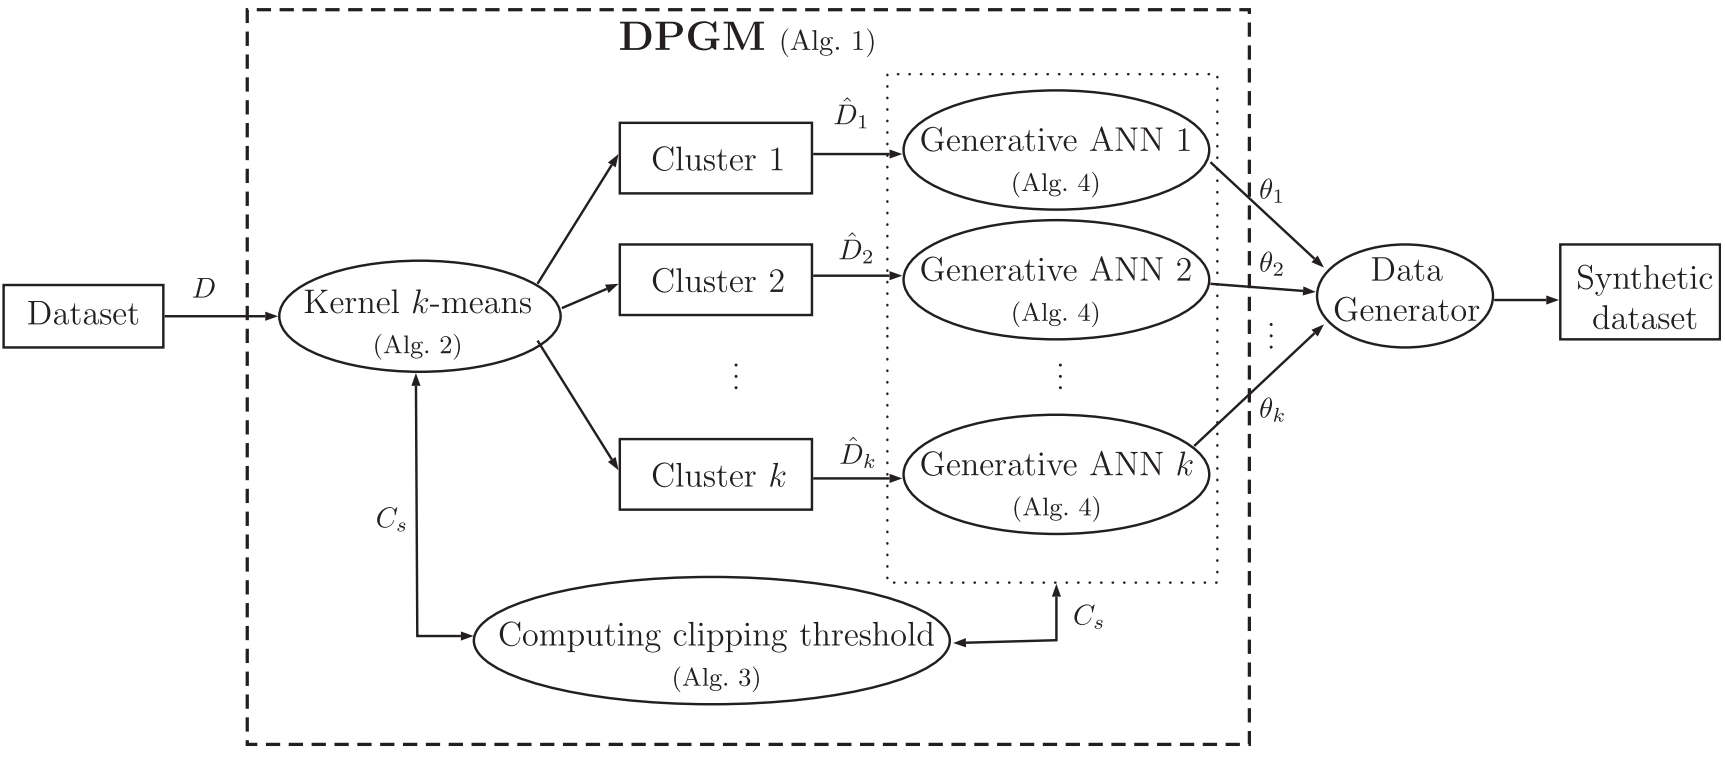
\includegraphics[width=0.5\textwidth,height=0.25\textwidth]{DP-GM.png}}
    \caption{The Overview of DP-GM.}
    \label{fig12}
\end{figure}\\
P3GM\cite{b49} divides the training of VAE into two phrases that are training the encoder and training the decoder with the fixed encoder and this increases the robustness against the noise for differential privacy protection. During the encoding phrase, PCA is first applied on the data to do dimension reduction for the simplification of encoding and then  noise following the Wishart mechanism is added to the covariance matrix to keep privacy preserving, and then EM-algorithm leading to some fixed parameters of encoder is done to obtain the estimation the distribution of the latent variable which is represented as the mixture of Gaussian in fact to approximate the prior distribution of real data with the differential privacy technique that is adding the noise sampled from the Gauss Mechanism with the sensitivity of dataset into the parameters. And when it comes to the decoding phrase, unfixed parameters of the encoder and all of the decoder are optimized following the AEVB algorithm which is the basic of VAE using a technique of Monte Carlo estimate to approximate the log-liklihood of posterior distribution with DP-SGD where the randomized gradient is crafted through computing the average over
the clipped gradients and adding noise from Gauss distribution to provide differential privacy.

\begin{figure}[htbp]
    \centerline{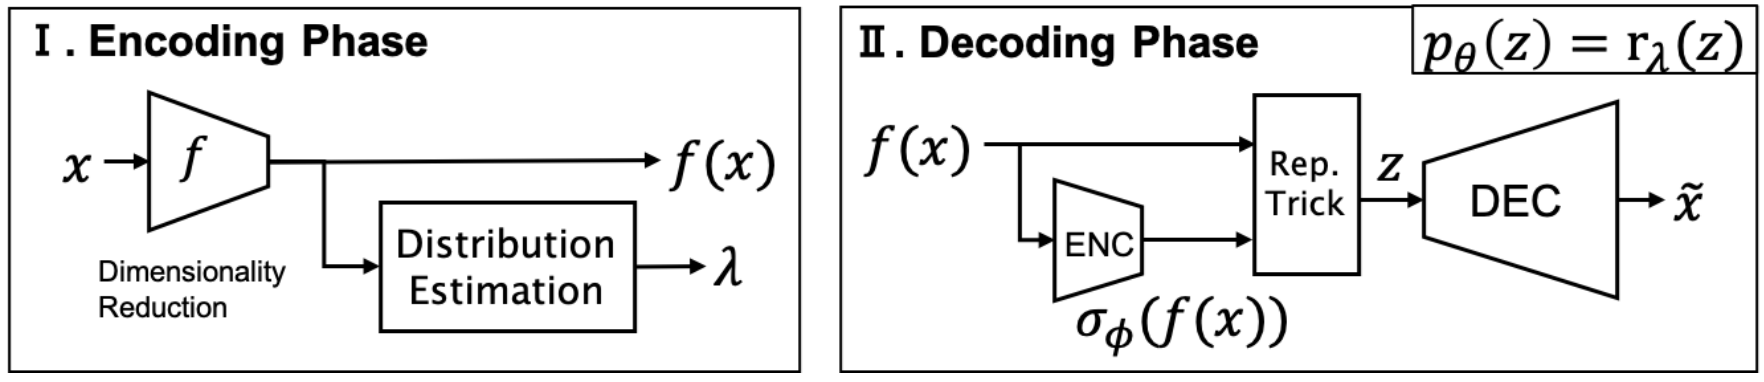
\includegraphics[width=0.4\textwidth,height=0.15\textwidth]{P3GM.png}}
    \caption{The Model Structure of P3GM.}
    \label{fig13}
\end{figure}





From above, it can be seen that the differential privacy combined with generative models have been explored a lot but there is still space for further study especially on other models except GAN, and DP-SGD is such a popular tool for differential privacy in the generative models but still need modification to perform tightly privacy budget suitable for different scenarios.


\section{Challenge}

\section{Conclusion}


\begin{thebibliography}{00}
\bibitem{b1} S. Sangeetha, G. Sudha Sadasivam, Privacy of Big Data: A Review, In: Dehghantanha, A., Choo, KK. (eds) Handbook of Big Data and IoT Security. Springer, Cham, 2019.
\bibitem{b2} C. Dwork and A. Roth. The algorithmic foundations of differential privacy. Foundations and Trends in Theoretical Computer Science, 9(3–4):211–407, 2014.
\bibitem{b3} Z. Sun, Y. Wang, M. Shu, el at., Differential Privacy for Data and Model Publishing of Medical Data, in IEEE Access, vol. 7, pp. 152103-152114, 2019.
\bibitem{b4} Y. Zhang, Z. Hao and S. Wang, A Differential Privacy Support Vector Machine Classifier Based on Dual Variable Perturbation, in IEEE Access, vol. 7, pp. 98238-98251, 2019.
\bibitem{b5} Huu Hiep Nguyen, Privacy-preserving mechanisms for k-modes clustering, Computers and Security, Volume 78, Pages 60-75, 2018.
\bibitem{b6}W. Rong, C.M. Fung Benjamin, Z. Yan, Heterogeneous data release for cluster analysis with differential privacy, Knowledge-Based Systems, Volumes 201–202, 2020.
\bibitem{b7} F. Ferdinando, H. Pascal V., Z. Keyu, Differential privacy of hierarchical Census data: An optimization approach, Artificial Intelligence, Volume 296, 103475, 2021.
\bibitem{b8} S. Haipei, X. Xiaokui, K. Issa, el at. Analyzing Subgraph Statistics from Extended Local Views with Decentralized Differential Privacy. In Proceedings of the 2019 ACM SIGSAC Conference on Computer and Communications Security (CCS '19). Association for Computing Machinery, New York, NY, USA, 703–717, 2019.
\bibitem{b9} H. Huang, D. Zhang, F. Xiao, el at, Privacy-Preserving Approach PBCN in Social Network With Differential Privacy, in IEEE Transactions on Network and Service Management, vol. 17, no. 2, pp. 931-945, June 2020.
\bibitem{b10} P. Tang, X. Cheng, S. Su, el at, Differentially Private Publication of Vertically Partitioned Data, in IEEE Transactions on Dependable and Secure Computing, vol. 18, no. 2, pp. 780-795, 1 March-April 2021.
\bibitem{b11} G. Maoguo, P. Ke, X. Yu, Differential privacy preservation in regression analysis based on relevance, Knowledge-Based Systems, Volume 173, Pages 140-149, 2019.
\bibitem{b12} X. Fang, F. Yu, G. Yang and el at, Regression Analysis With Differential Privacy Preserving, in IEEE Access, vol. 7, pp. 129353-129361, 2019.
\bibitem{b13} P. Ke, G. Maoguo, F. Kaiyuan, el at, Differentially private regression analysis with dynamic privacy allocation, Knowledge-Based Systems, Volume 217, 106795, 2021.
\bibitem{b14} L. Katrina, N. Seth, R. Aaron, el at, Accuracy first: selecting a differential privacy level for accuracy-constrained ERM. In Proceedings of the 31st International Conference on Neural Information Processing Systems (NIPS'17). Curran Associates Inc., Red Hook, NY, USA, 2563–2573, 2017.
\bibitem{b15} M. Abadi, A. Chu, I. Goodfellow, el at, Deep Learning with Differential Privacy, In Proceedings of the 2016 ACM SIGSAC Conference on Computer and Communications Security (CCS '16). Association for Computing Machinery, New York, NY, USA, 308–318, 2016.
\bibitem{b16} Anda C., Jiaxing W., Z. X. Sheryl, el at, DPNAS: Neural Architecture Search for Deep Learning with Differential Privacy. Proceedings of the AAAI Conference on Artificial Intelligence, 36(6), 6358-6366, 2022.
\bibitem{b17} P. Nicolas, T. Abhradeep, S. Shuang, el at, Tempered Sigmoid Activations for Deep Learning with Differential Privacy. Proceedings of the AAAI Conference on Artificial Intelligence, 35(10), 9312-9321, 2021.
\bibitem{b18} Y. Da, Z. Huishuai, C. Wei, el at, Do Not Let Privacy Overbill Utility: Gradient Embedding Perturbation for Private Learning. International Conference on Learning Representations (ICLR), 2021.
\bibitem{b19} Z. Yingxue, W. Steven, B. Arindam, Bypassing the Ambient Dimension: Private SGD with Gradient Subspace Identification. International Conference on Learning Representations (ICLR), 2021
\bibitem{b20} M. H. Brendan, R. Daniel, T. Kunal, el at, Learning Differentially Private Recurrent Language Models, 6th International Conference on Learning Representations(ICLR 2018) - Conference Track Proceedings, 2018.
\bibitem{b21} A. Naman, S. A. Theertha, Y. Felix, el at, CpSGD: communication-efficient and differentially-private distributed SGD. In Proceedings of the 32nd International Conference on Neural Information Processing Systems (NIPS'18). Curran Associates Inc., Red Hook, NY, USA, 7575–7586, 2018.
\bibitem{b22} N. Phan, X. Wu, H. Hu and D. Dou, Adaptive Laplace Mechanism: Differential Privacy Preservation in Deep Learning, 2017 IEEE International Conference on Data Mining (ICDM), pp. 385-394, 2017.
\bibitem{b23} P. Nicolas, G. Ian, A. Martín, el at, Semi-supervised Knowledge Transfer for Deep Learning from Private Training Data, 5th International Conference on Learning Representations(ICLR 2017) - Conference Track Proceedings, 2017.
\bibitem{b24} P. Nicolas, S. Shuang, M. Ilya, el at., Scalable Private Learning with PATE, 6th International Conference on Learning Representations(ICLR 2018) - Conference Track Proceedings, 2018.
\bibitem{b25} L. Lingjuan  and C. Chihua, Differentially Private Knowledge Distillation for Mobile Analytics, In Proceedings of the 43rd International ACM SIGIR Conference on Research and Development in Information Retrieval (SIGIR '20). Association for Computing Machinery, New York, NY, USA, 1809–1812, 2020. 
\bibitem{b26} L. Yin, J. Feng, H. Xun, el at., A Privacy-Preserving Federated Learning for Multiparty Data Sharing in Social IoTs, in IEEE Transactions on Network Science and Engineering, vol. 8, no. 3, pp. 2706-2718, 1 July-Sept. 2021.
\bibitem{b27} Y. Guo and Y. Gong, Practical Collaborative Learning for Crowdsensing in the Internet of Things with Differential Privacy, 2018 IEEE Conference on Communications and Network Security (CNS), pp. 1-9, 2018.
\bibitem{b28} W. Xiang, Z. Yongting, S. Minyu, el at., An adaptive federated learning scheme with differential privacy preserving, Future Generation Computer Systems, Volume 127, Pages 362-372, 2022.
\bibitem{b29} Raef Bassily, Linear Queries Estimation with Local Differential Privacy, Proceedings of the Twenty-Second International Conference on Artificial Intelligence and Statistics, PMLR 89:721-729, 2019.
\bibitem{b30} M. Bun, T. Steinke, Concentrated Differential Privacy: Simplifications, Extensions, and Lower Bounds. In: Hirt, M., Smith, A. (eds) Theory of Cryptography. TCC 2016. Lecture Notes in Computer Science(), vol 9985. Springer, Berlin, Heidelberg, 2016.
\bibitem{b31} 
I. Mironov, Rényi Differential Privacy, 2017 IEEE 30th Computer Security Foundations Symposium (CSF), pp. 263-275, 2017.
\bibitem{b32} 
G. Ian J., P. Jean , M. Mehdi, el at, Generative Adversarial Nets, Advances in Neural Information Processing Systems (NIPS'14), 2014.
\bibitem{b33} K. Diederik P., W. Max, Auto-Encoding Variational Bayes, 2nd International Conference on Learning Representations(ICLR 2014) - Conference Track Proceedings, 2014.
\bibitem{b34} J. James, Y. Jinsung, S. Mihaela V. D., PATE-GAN: Generating Synthetic Data with Differential Privacy Guarantees, 7th International Conference on Learning Representations, ICLR 2019 (2019)
\bibitem{b35} L. Yunhui, W. Boxin, Y. Zhuolin, et al. G-PATE: Scalable Differentially Private Data Generator via Private Aggregation of Teacher Discriminators, Advances in Neural Information Processing Systems (NIPS'21), 2021.
\bibitem{b36} F. Lorenzo, O. Anderson S. de, G. Laurent, el at., Differentially Private Generative Adversarial Networks for Time Series, Continuous, and Discrete Open Data, ICT Systems Security and Privacy Protection. SEC 2019. IFIP Advances in Information and Communication Technology, vol 562. Springer, Cham, 2019.
\bibitem{b37}X. Chugui, R. Ju, Z. Deyu, el at., GANobfuscator: Mitigating Information Leakage Under GAN via Differential Privacy, in IEEE Transactions on Information Forensics and Security, vol. 14, no. 9, pp. 2358-2371, Sept. 2019.
\bibitem{b38} T. Reihaneh,  K. Peter and P. Benedict, DP-CGAN: Differentially Private Synthetic Data and Label Generation, 2019 IEEE/CVF Conference on Computer Vision and Pattern Recognition Workshops (CVPRW),  pp. 98-104, 2019.
\bibitem{b39} H. Stella, Q. Youyang, G. Longxing, el at., Generative Adversarial Nets Enhanced Continual Data Release Using Differential Privacy, Algorithms and Architectures for Parallel Processing. ICA3PP 2019. Lecture Notes in Computer Science(), vol 11945, Springer, Cham, 2020.
\bibitem{b40} Q. Youyang, Y. Shui, Z. Jingwen, el.at., GAN-DP: Generative Adversarial Net Driven Differentially Privacy-Preserving Big Data Publishing, ICC 2019 - 2019 IEEE International Conference on Communications (ICC), 2019, pp. 1-6, 2019.
\bibitem{b41} C. Dingfan, O. Tribhuvanesh, and F. Mario, GS-WGAN: A Gradient-sanitized Approach for Learning Differentially Private generators. Advances in Neural Information Processing Systems 33 (NIPS'20), 2020.
\bibitem{b42} S. Augenstein, H. B. McMahan, D. Ramage, el at., Generative Models for Effective ML on Private, Decentralized Datasets, In International Conference on Learning Representations (ICLR), 2020.
\bibitem{b43} Trung H. and D. Tran K., Investigating Local Differential Privacy and Generative Adversarial Network in Collecting Data, International Conference on Advanced Computing and Applications (ACOMP) 2020, pp. 140-145, 2020
\bibitem{b44} Xikun J., Chaoyue N., Chenhao Y., el at., Pricing GAN-based data generators under Rényi differential privacy, Information Sciences, Volume 602, Pages 57-74, 2022.
\bibitem{b45} C. William L., S. Jörg-Rüdiger, S. Wei, Differentially private facial obfuscation via generative adversarial networks,
Future Generation Computer Systems, Volume 129, Pages 358-379, 2022.
\bibitem{b46} Benjamin W., Valentin R., Michael A., el at.,  DP-VAE: Human-Readable Text Anonymization for Online Reviews with Differentially Private Variational Autoencoders, In Proceedings of the ACM Web Conference 2022 (WWW '22), Association for Computing Machinery, New York, NY, USA, 721–731, 2022.
\bibitem{b47} Le F., Bingqian D. and Chuan W., Differentially private recommender system with variational autoencoders, Knowledge-Based Systems, Volume 250, 109044, 2022.
\bibitem{b48} Gergely A., Luca M., Claude C., el at., Differentially Private Mixture of Generative Neural Networks, in IEEE Transactions on Knowledge and Data Engineering, vol. 31, no. 6, pp. 1109-1121, 2019.
\bibitem{b49} T. Shun, T. Tsubasa, C. Yang, el at., P3GM: Private High-Dimensional Data Release via Privacy Preserving Phased Generative Model, 2021 IEEE 37th International Conference on Data Engineering (ICDE), 2021, pp. 169-180, 2022.

\end{thebibliography}

\end{document}
